\begin{figure}[h]
  \begin{center}
  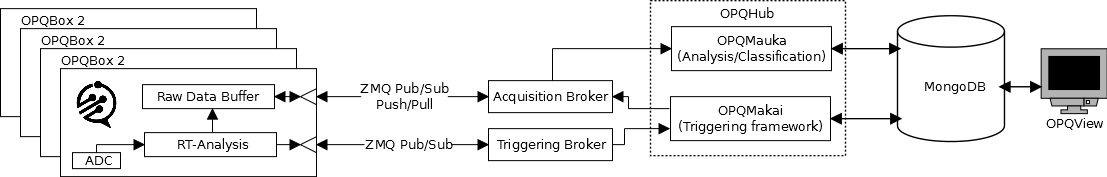
\includegraphics[width=0.9\textwidth]{img/system-diagram.png}
  \end{center}
  \caption{Block diagram of the OPQ Power Quality monitoring system.}
  \label{fig:opq:1}
\end{figure}

The Open Power Quality (OPQ) power quality monitoring network utilizes residential power quality meters, called OPQ Boxes, in order to detect anomalies in the electricity distribution across the Oahu power grid.
In addition to OPQ Boxes, the OPQ project utilizes cloud-based aggregation services for power quality event detection, classification and display.
The block diagram of the OPQ network is shown in Figure~\ref{fig:opq:1} .

The major components of OPQ are:
\begin {itemize}
	\item OPQ Box: An open source power quality meter which conforms to Napali Framework requirements for the "source".
	\item Makai: data aggregation and event detection service that I designed and that runs as part of the sensor network "sink".
	\item Mauka: event analysis and classification service designed by my colleague Anthony Christe.
\end {itemize}

The following sections describe the OPQ network components, services and protocols.

\section{OPQ Box}\label{sec:opq-box}

OPQ Box is a power quality meter I designed for the OPQ project, which focuses on providing the means for cheap, extensible and accurate residential power quality measurements.
The block diagram of the current revision of OPQ Box, OPQ Box2 is shown in the Figure~\ref{fig:opq:1:1}.
A complete device is shown in Figure~\ref{fig:opq:1:2}.

\begin{figure}[h]
	\centering
	\begin{subfigure}{.5\textwidth}
	  \centering
	  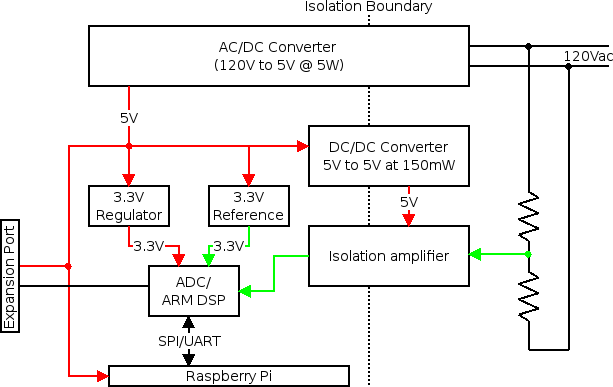
\includegraphics[width=0.9\linewidth]{img/opqbox_diagram.png}
	  \caption{OPQ Box2 Block Diagram.
	  The power path is in red, signal path is in green and the digital IO is in black.}
	  \label{fig:opq:1:1}
	\end{subfigure}%
	\begin{subfigure}{.5\textwidth}
	  \centering
	  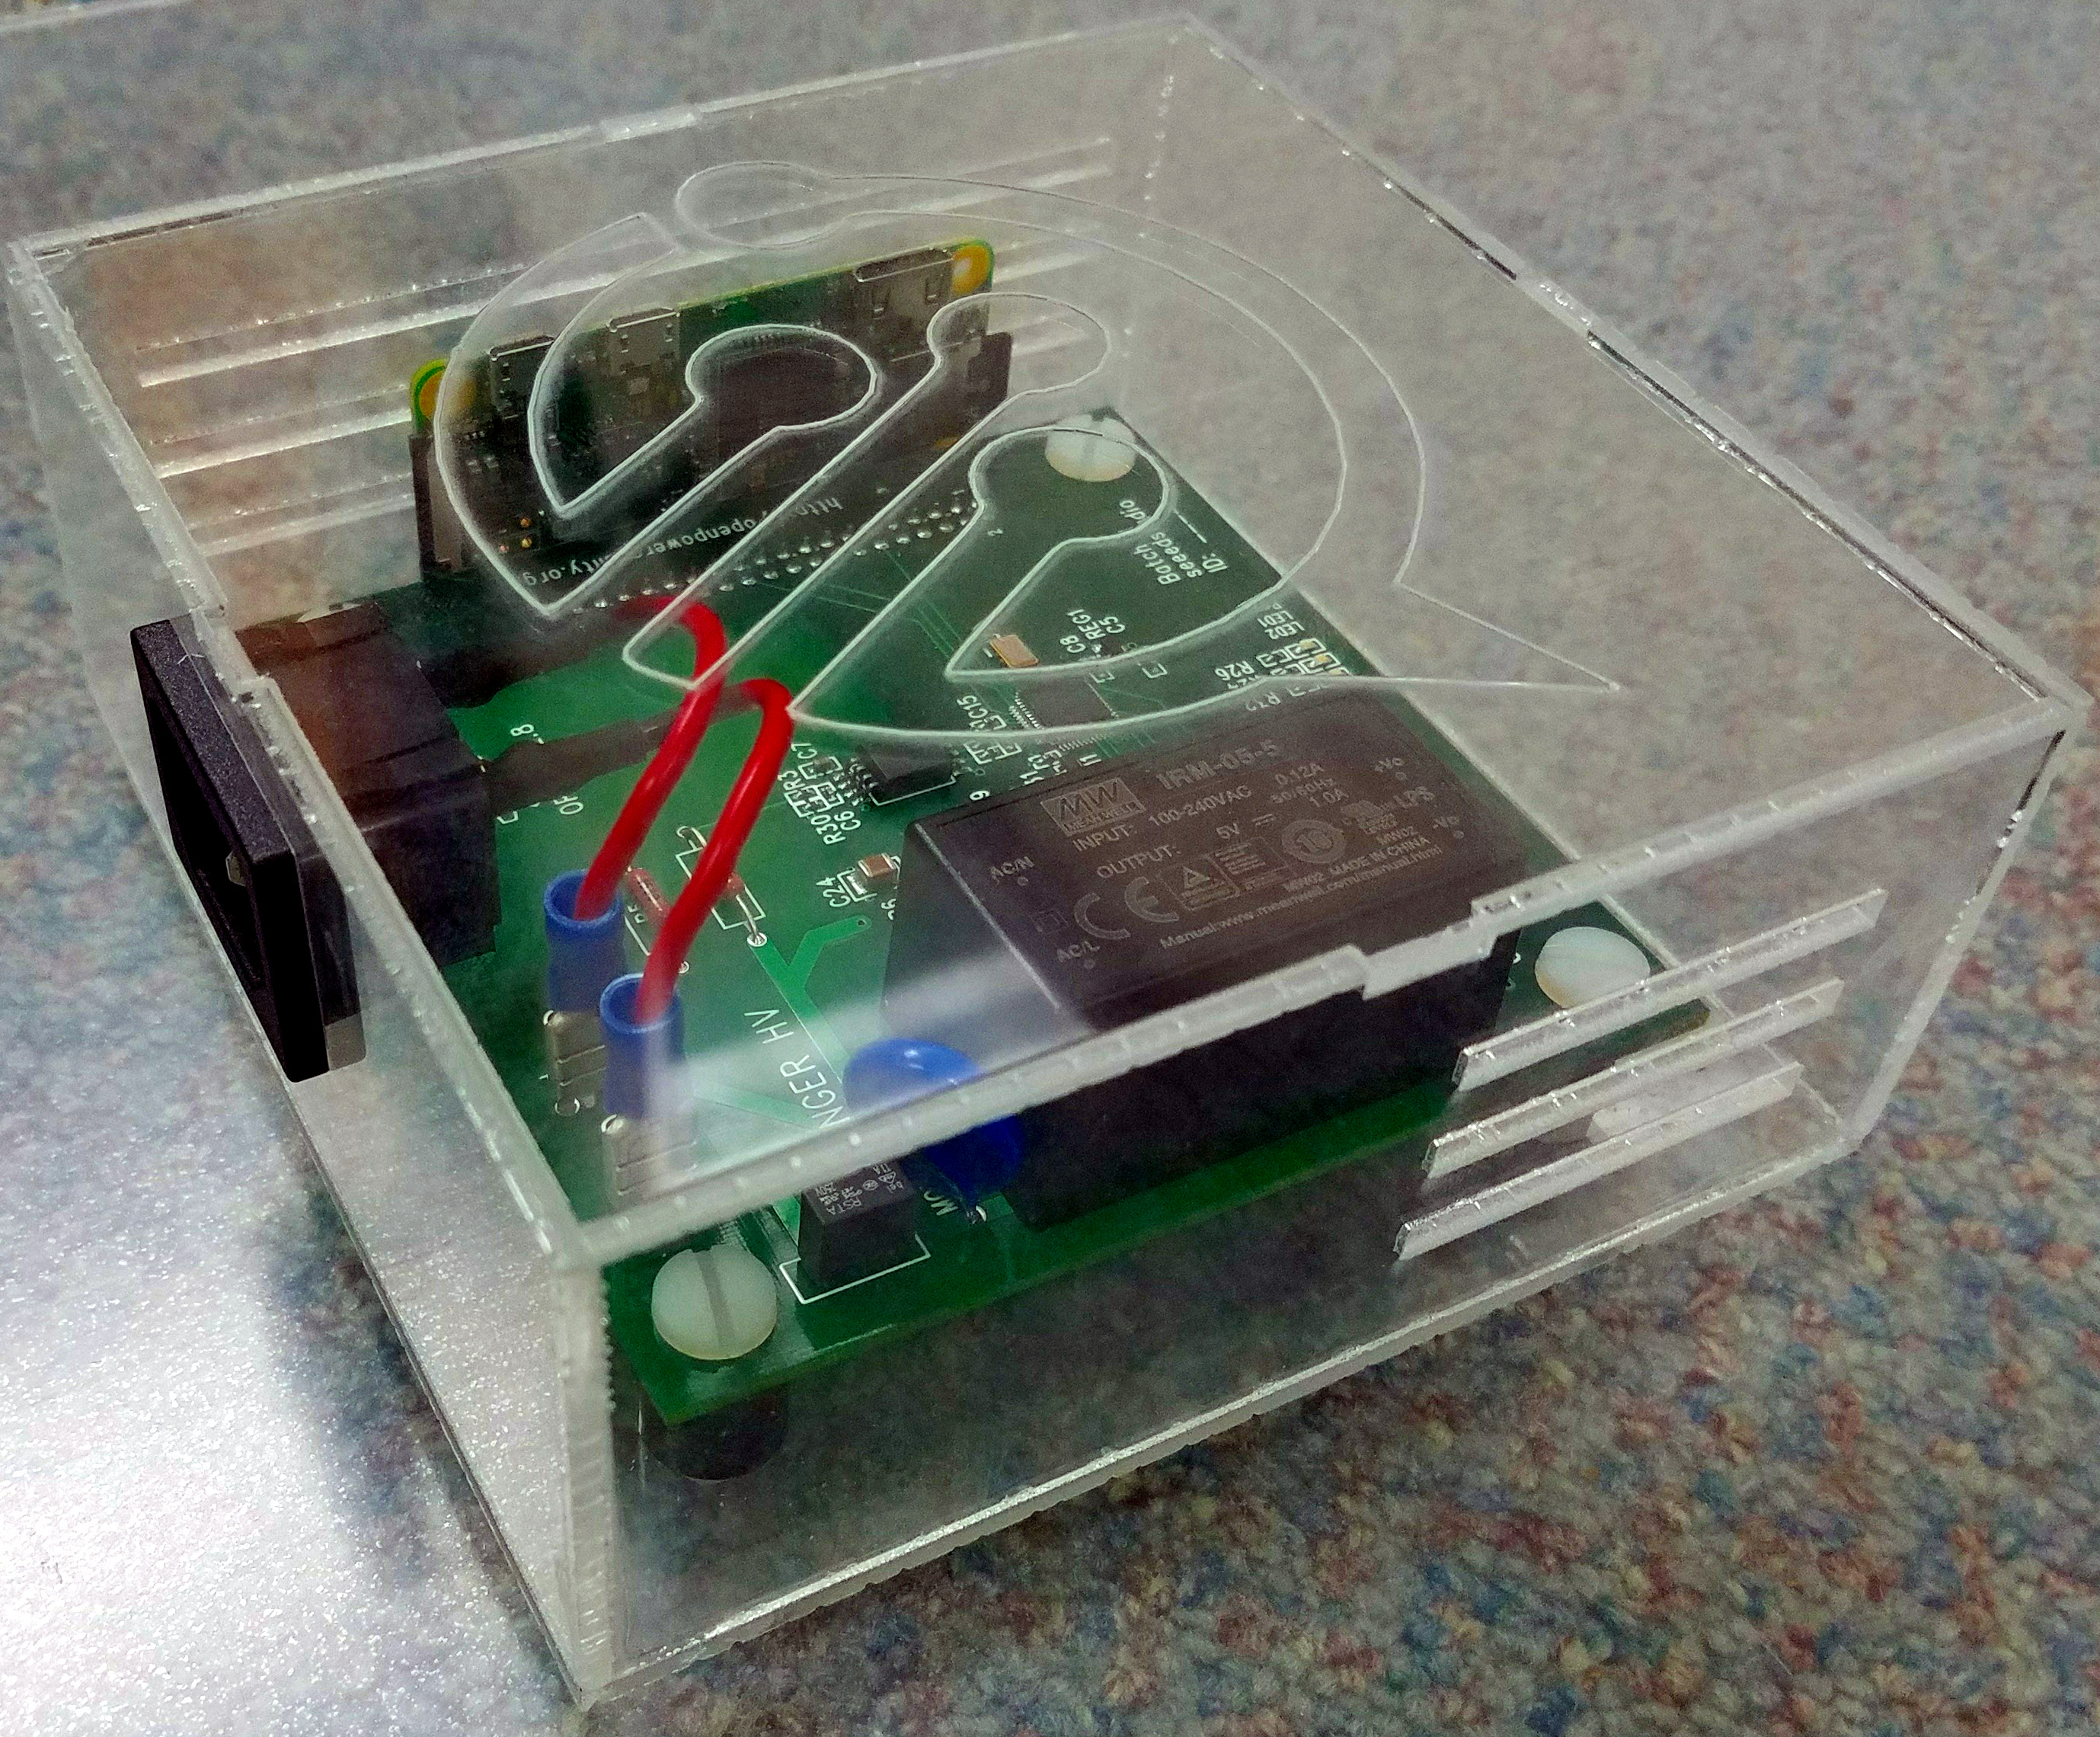
\includegraphics[width=0.7\linewidth]{img/opqbox_photo.jpg}
	  \caption{OPQ Box2 in an acrylic enclosure.}
	  \label{fig:opq:1:2}
	\end{subfigure}
	\caption{(a) OPQ Box2 block diagram and (b) production OPQ Box ready for deployment}
	\label{fig:opq:2}
\end{figure}

\subsection{Hardware}\label{subsec:hardware}

The power system of the OPQ Box2 electrically isolates most of the device from the AC mains power.
An isolated AC-DC converter generates $5V_{dc}$ from the mains $120V_{ac}$.
5V is used to power the Raspberry Pi, equipment connected to the expansion port, 3.3V regulators and voltage reference and an isolated DC/DC converter.
3.3V is used to power the isolated end of the isolation amplifier as well as the STM32F3 analog to digital converter/digital signal processor (ADC/DSP).
The hot side of the isolation amplifier is powered from the isolated DC/DC converter.
This allows OPQ Box to function with the battery attached to the expansion port, so that it may retain data and continue to operate during a power outage.


The analog signal path of the OPQ Box2 is complicated by the fact that the STM32F3 ADC/DSP is electrically isolated from the mains power.
A previous iteration of the OPQ Box, OPQ Box1, overcame this by employing small circuit board mount isolation transformer.
Unfortunately it was found that the frequency response of these transformers varied wildly between individuals, thus incurring a lengthy calibration process for each device.
Design on the OPQ Box2 solved this issue by using an AMC1100 isolation amplifier as the isolation component.
Internally AMC1100 consists of a single die comprised of a $\Sigma\Delta$ analog to digital and digital to analog converters.
These converters are separated by a silicon glass region on the integrated circuit which acts as a coupling capacitor.
Since the signal passes the isolation boundary as a $\Sigma\Delta$ encoded digital signal, it incurs no distortion and no additional calibration is required.
In order to match the dynamic range of the AMC1100 the $120V_{ac}$ is passed through the resistor divider to attenuate it to $120mV_{ac}$.
The input and output of the isolation amplifier is filtered with a passive first order anti-aliasing filter.
Isolated signal is then digitized via a 16bit ADC of the STM32F3 DSP at $12 KSps$, which gives 200 data samples per grid cycle.
Internally digitization process runs asynchronously with the respect to the the DSP CPU, in order to minimize timing jitter.
It was verified that the sampling jitter of the ADC is less then 1us, however due to limited precision of equipment an exact figure was not established.
Data stream in its digital form is transferred to the Raspberry Pi single board computer (SBC) for analysis.

\begin{figure}[h]
  \begin{center}
  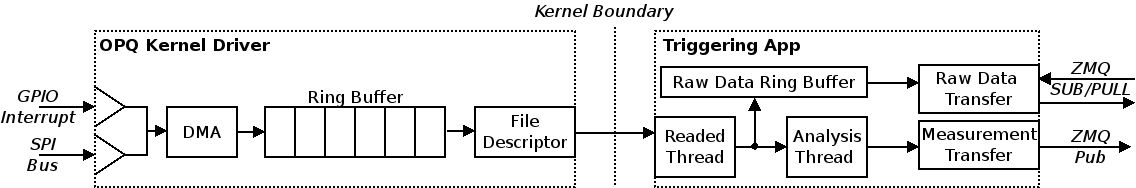
\includegraphics[width=0.9\textwidth]{img/opqbox_software.png}
  \end{center}
  \caption{Block diagram of the OPQ Box 2 software stack.}
  \label{fig:opq:3}
\end{figure}

Raspberry Pi SBC is responsible for signal analysis and anomaly detection.
The Raspberry Pi model used in OPQ Box is the Pi Zero W equipped with 256MB of main memory and a single core 1GHz ARM11 CPU. Furthermore, Pi Zero W is equipped with an on-board 802.11n WIFI transceiver, which removes the need for an external WIFI dongle used in previous OPQ Box devices.
\subsection{Software}\label{subsec:software}
The software stack of the Raspberry Pi aims to deliver a full featured power quality analysis framework despite its rather limited hardware capabilities.
A block diagram of the software stack is shown in Figure~\ref{fig:opq:3}.
Digital data is transferred from the DSP to the Raspberry Pi via Serial Peripheral Interface, with the Pi acting as the master and the DSP as a slave device.
A hardware interrupt line is used to inform Pi software that the DSP is ready for the data transfer.
During the initial design of the OPQ Box 2 software, SPI data transfer was attempted in userland.
However due to the lack of support for DMA in the SPI kernel-to-userland bridge, a large portion of the CPU time was spent facilitating data transfer, resulting in degraded analysis performance as well as missed data samples.
Current revision of the OPQ Box 2 software stack utilizes a kernel driver for management of SPI bus.
Internally OPQ driver maintains a ring buffer of 16 windows each 200 data samples in size.
Upon the receiving the interrupt for the DSP, the CPU sets up the DMA transfer and the DMA engine transfers a 200 sample window into the kernel memory without CPU interaction.
This scheme requires the CPU to only service 60 interrupts a second, with each interrupt requiring on the order of 100 instructions, yielding the CPU utilization of less then $1\%$ in normal operation.
Userland applications communicate with the kernel driver using a file descriptor, where every $write$ system call yields 200 samples of raw waveform.
Thus the smallest window that a userland application may process is a single AC cycle of the grid mains.

Userland component of the OPQ Box 2 software is a multi-threaded extensible analysis framework called Triggering.
The reader thread is responsible for transferring and accumulating data from the kernel driver.
The smallest data buffer that the Triggering application processes at any given time is 10 grid cycles or 2k samples.
Once the cycles are transferred to the userland and timestamped, they are passed to the analysis thread for feature extraction, as well as to the Raw Data Ring Buffer (RDRB).
Since internally all data is addressed using shared pointers, during data duplication no copying is required.
RDRS is capable of buffering up to an hour of historic data before it's overwritten resulting in the RDBS maximum size of 100MB.

Analysis thread of the Triggering application performs feature extraction of the raw data windows of 2000 samples.
Four metrics are extracted from the data stream:
\begin{itemize}
	\item Fundamental frequency.
	\item RMS Voltage.
	\item Total Harmonic Distortion.
	\item Transient.
\end{itemize}

\subsection{Fundamental Frequency}\label{subsec:fundamental-frequency}

Fundamental frequency is calculated by computing the zero crossings of the AC waveform.
Since a sinusoid has two zero crossings for a full cycle the frequency can be calculated as:
\begin{equation} \label{eq:1}
 f = \frac{1}{\frac{2}{n}\sum\limits_{k=0}^{k=n}{\Delta t_{k}}}
\end{equation}

\begin{figure}[h]
	\centering
	\begin{subfigure}{.5\textwidth}
	  \centering
	  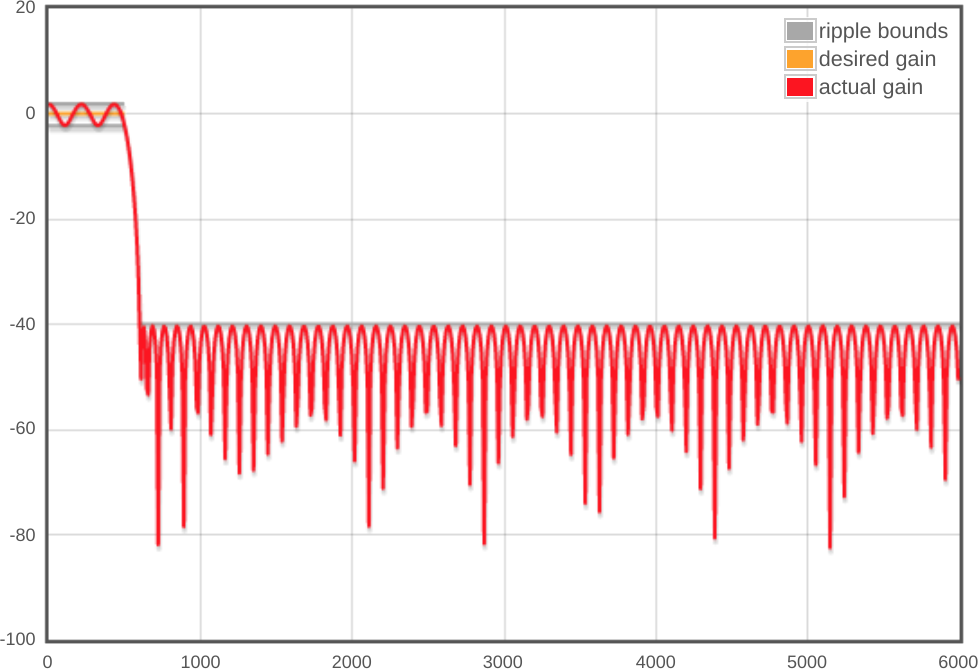
\includegraphics[width=0.9\linewidth]{img/filter1_gain.png}
	  \caption{}
	  \label{fig:opq:4:1}
	\end{subfigure}%
	\begin{subfigure}{.5\textwidth}
	  \centering
	  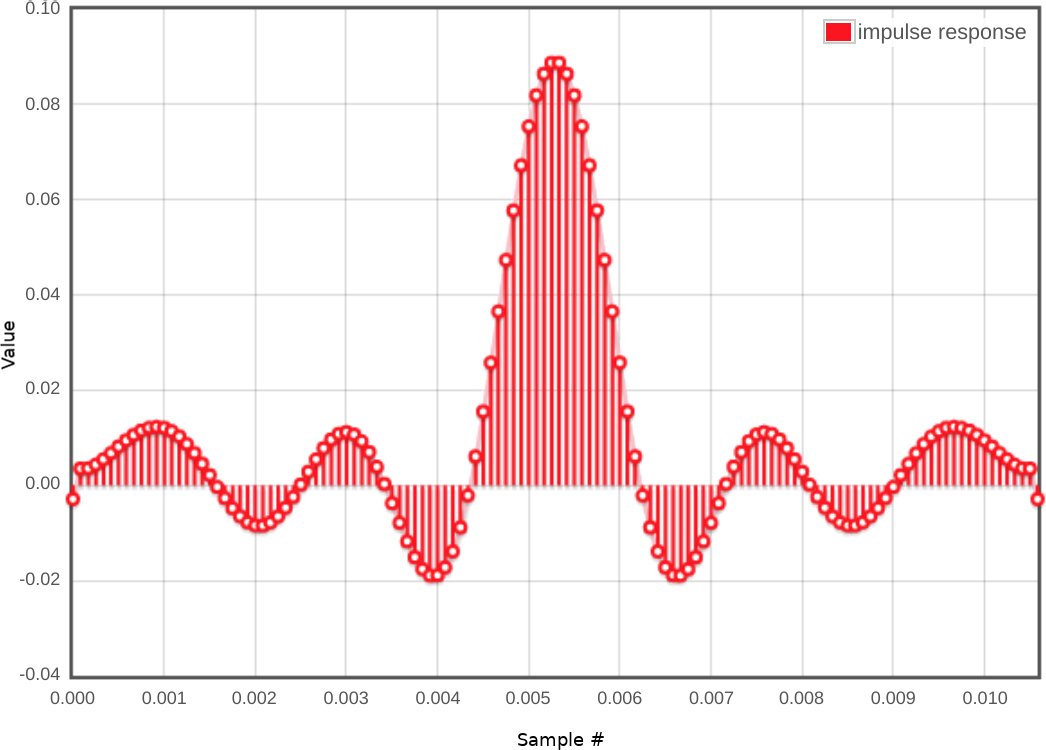
\includegraphics[width=0.9\linewidth]{img/filter1_response.png}
	  \caption{}
	  \label{fig:opq:4:2}
	\end{subfigure}

	\begin{subfigure}{.5\textwidth}
	  \centering
	  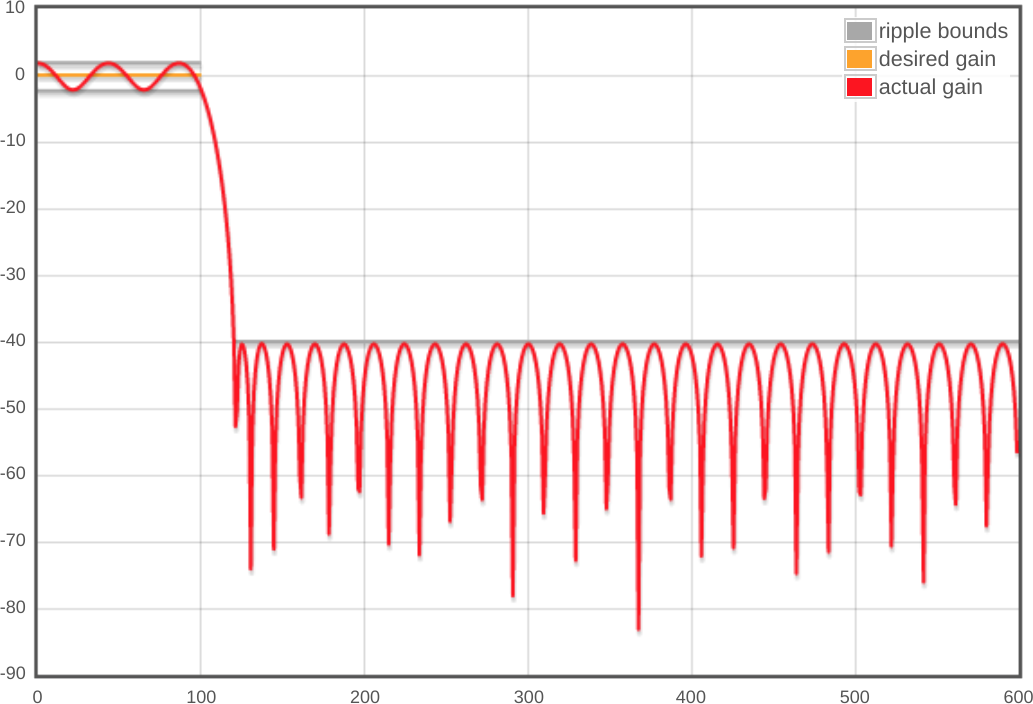
\includegraphics[width=0.9\linewidth]{img/filter2_gain.png}
	  \caption{}
	  \label{fig:opq:4:3}
	\end{subfigure}%
	\begin{subfigure}{.5\textwidth}
	  \centering
	  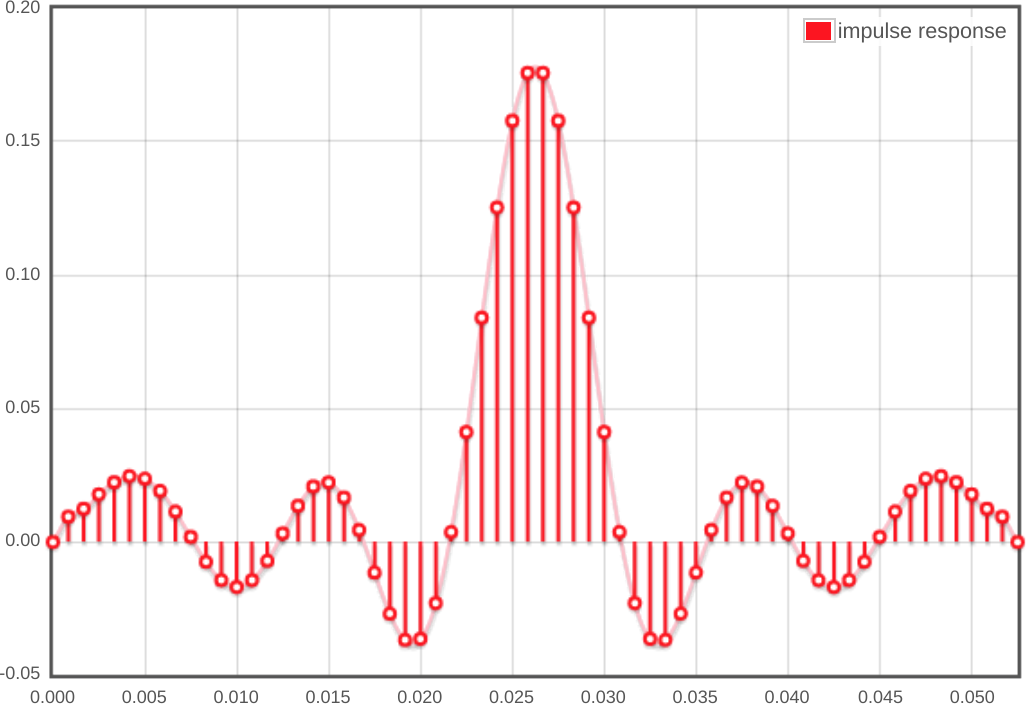
\includegraphics[width=0.9\linewidth]{img/filter2_response.png}
	  \caption{}
	  \label{fig:opq:4:4}
	\end{subfigure}
	\caption{Filters used for mains frequency calculation. (a) Downsampling filter gain. (b) Downsampling filter impulse response. (c) Lowpass filter gain. (d) Lowpass filter impulse response.}
	\label{fig:opq:4}
\end{figure}

Where the $\Delta t_{k}$ is the k'th time between two adjacent zero crossings.
In order to improve the accuracy of the frequency calculation one must first filter out as much noise as possible.
Since our sampling rate is quite high (12kSps) and the fundamental frequency is quite low (60Hz) it is very computationally expensive to perform this filtering in a single step.
Instead filtering is accomplished via a set of two finite impulse response (FIR) filters shown in Figure~\ref{fig:opq:4:2} and~\ref{fig:opq:4:4}.
First the Down sampling filter is applied to the raw waveform, which results in the frequency response shown in Figure~\ref{fig:opq:4:1}.
As is evident by the plot the frequency content of the result is 0-600Hz, Thus it can be downsampled to the $\frac{N}{10}$, or 200 samples without aliasing.
Next the low pass filter is applied to the downsampled waveform with the frequency response shown in Figure~\ref{fig:opq:4:3}.This resulting frequency content is 0-100Hz, thus all of the higher frequency harmonics and noise are removed.
Finally the twice filtered downsampled waveform is used to estimate the fundamental frequency according to the Equation~\ref{eq:1}.
The zero crossings themselves were calculated by using linear interpolation between two points which bracket the time axis.

All electrical generation systems connected to the grid run synchronously with each other, meaning that while small variations in voltage are common across locations, the fundamental frequency and phase must remain strictly in sync.
This effect is demonstrated in Figure~\ref{fig:opq:5}, which is a frequency fluctuation event recorded on November 8 2017.
While the two devices were separated by ten miles, their frequency measurements track closely together.

\begin{figure}[h]
	\centering
	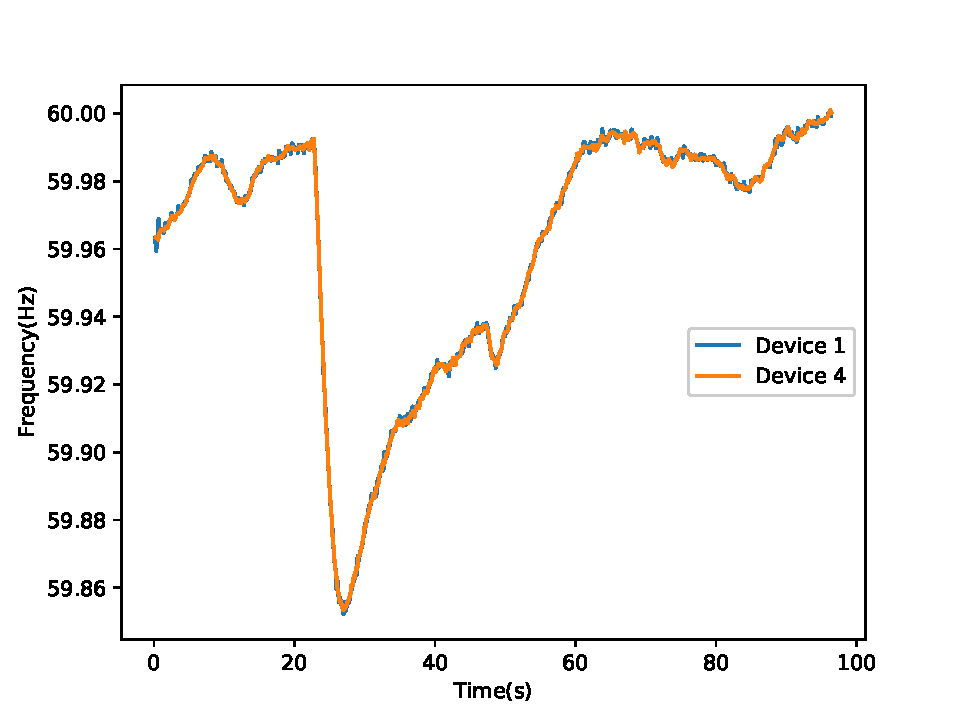
\includegraphics[width=0.6\linewidth]{img/frequency_two_devices.pdf}
	\caption{Frequency measurement across two devices recorded during a lighting strike.}
	\label{fig:opq:5}
\end{figure}

\subsection{Root Mean Square Voltage}\label{subsec:root-mean-square-voltage}

Root mean square voltage ($V_{rms}$) in electrical power is the equivalent value of DC voltage which would dissipate the same power in the resistive load. $V_{rms}$ is a convenient measure for detecting voltage sags and swells, since they result in nominally higher and lower computed value.
For the sinusoidal signal $V_{rms}$ can be calculated from the peak to peak value ($V_{pp}$) as:
\begin{equation} \label{eq:2}
	V_{rms} = \frac{V_{pp}}{2\sqrt{2}}
\end{equation}
It is common for multimeter to employ the equation above for computing $V_{rms}$.
However this equation is only valid for a perfect sinusoid, and thus does not result in a suitable metric for identifying power quality disturbances.
Instead OPQ Box 2 computes $V_{rms}$ as follows:
\begin{equation} \label{eq:3}
	V_{rms} = \sqrt{\frac{1}{n}\sum\limits_{k=0}^{k=n}V_{k}^{2}}
\end{equation}
Similarly to the frequency calculation OPQ Box 2 usees a 10 cycle window for a single $V_{rms}$ calculation, however unlike the frequency calculation the input is not filtered a priori.
An example of a power quality disturbance which exhibits low $V_{rms}$ is shown in Figure~\ref{fig:opq:6:1} and~\ref{fig:opq:6:2}.
These disturbances are the result of a lighting strike recorded by two OPQ Box 2 devices on Nov 1, 2017.

\begin{figure}[h]
		\centering
	\begin{subfigure}{.5\textwidth}
	  \centering
	  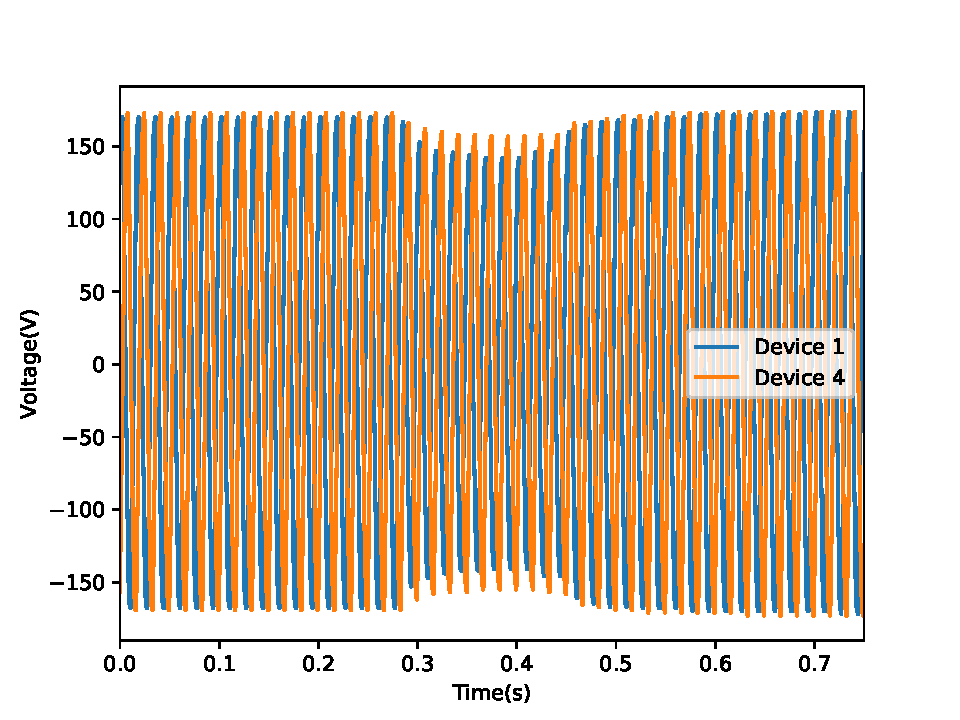
\includegraphics[width=0.9\linewidth]{img/voltage_sag.pdf}
	  \caption{}
	  \label{fig:opq:6:1}
	\end{subfigure}%
	\begin{subfigure}{.5\textwidth}
	  \centering
	  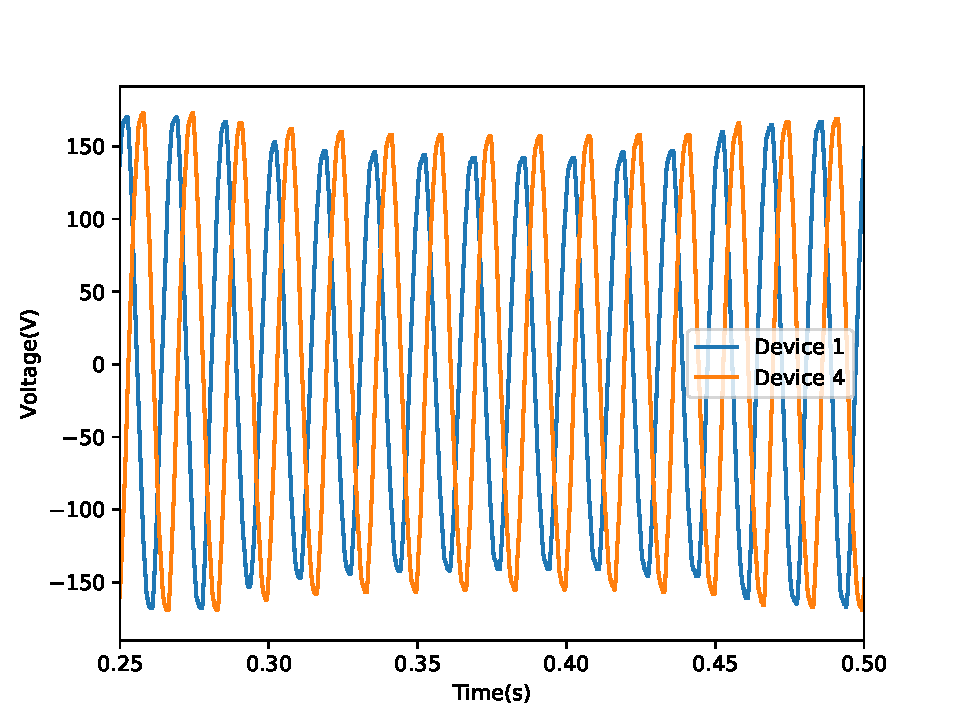
\includegraphics[width=0.9\linewidth]{img/voltage_sag_zoomed_in.pdf}
	  \caption{}
	  \label{fig:opq:6:2}
	\end{subfigure}
	\caption{A lightning strike recorded by two OPQ Box 2 devices separated by 10 miles. (a) A lightning strike manifested as $V_{rms}$ dip which lasted 11 cycles. (b) As a consequence of using NTP these devices have $\frac{1}{2}$ cycle mismatch in reported timestamps.}
	\label{fig:opq:6}
\end{figure}


\subsection{Total Harmonic Distortion}\label{subsec:thd}
OPQ Box calculates THD using industry standard methodology.
In the power delivery industry THD is defined as:
\begin{equation} \label{eq:4}
THD = \frac{\sqrt{\sum{V_{n}^2}}}{V_{f}}*100\%
\end{equation}
Where $V_{f}$ is the fundamental 60Hz power and $V_{n}$ is the power at $n^{th}$ harmonic.
It should be noted that in the power quality domain THD is expressed as a percentage as opposed to $\frac{dB}{\sqrt{Hz}}$ as used in other disciplines.
Operationally, OPQ Box computes THD for 10 cycles of the fundamental frequency.
First an FFT transforms the real voltage samples into it's frequency components.
Next, the square of the harmonic bins is accumulated and scaled by the magnitude of the fundamental power.

\begin{figure}[h]
	\centering
	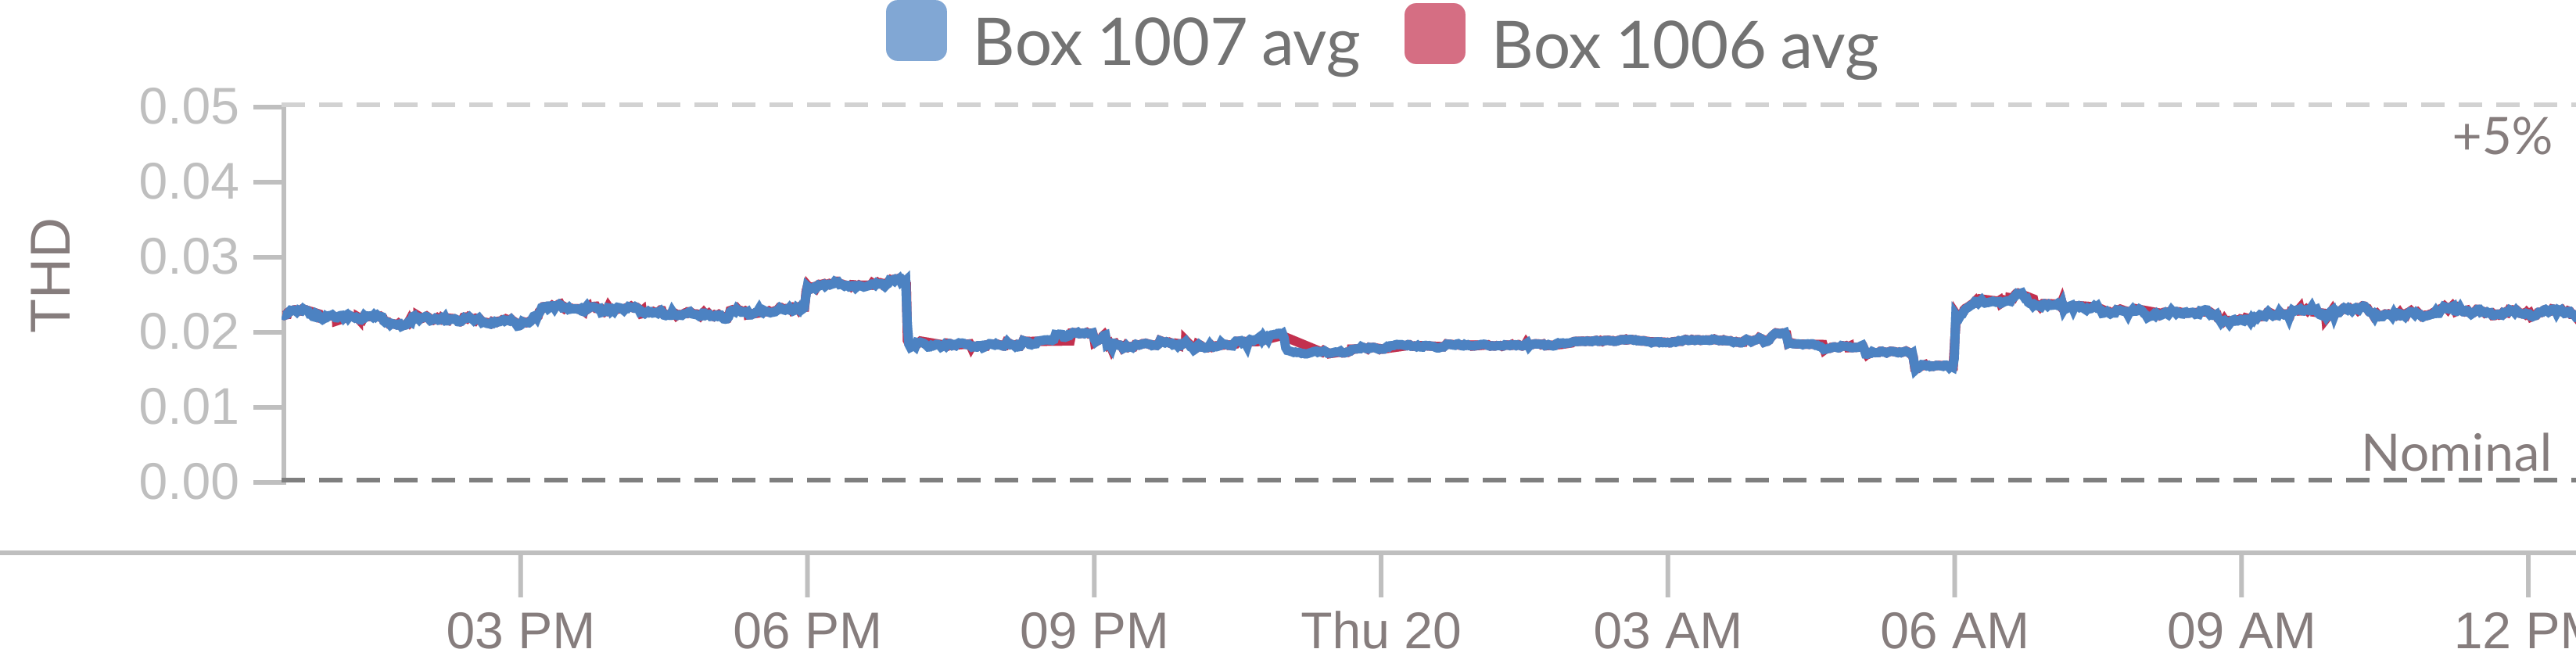
\includegraphics[width=1\linewidth]{img/thd_two_devices_24_hours.png}
	\caption{A common THD trend across two OPQ Box devices each deployed in the two Flexible Response to Ongoing Growth buildings on UH campus.}
	\label{fig:opq:7}
\end{figure}

Figure~\ref{fig:opq:7} shows a common trend observed by all OPQ Box devices installed on the UH campus.
For clarity only two devices are shown.
It is assumed that the large drop observed daily from approximately 6am to 6pm corresponds to the automatic response of the power delivery system to the reactive power in the grid, by deploying a large capacitor bank to compensate for the current phase lag.

\subsection{Transient Detection}\label{subsec:transient-detection}

OPQ Box transient detection is performed via filtering out of the fundamental frequency via an FIR high pass pass filter and searching for a maximum value in the remainder.
The high pass filter has a cutoff of $400Hz$, and the filter coefficients and response are shown in Figure~\ref{fig:opq:8:2} and Figure~\ref{fig:opq:8:1} respectively.
The result of the high pass filter operation is shown in Figure~\ref{fig:opq:8}.
Figure~\ref{fig:opq:8:3} shows a synthetic signal generated via a SDG1025 signal generator and fed into the OPQ Box.
This signal contains a $5V_{pp}$ transient injected at 11ms.
Filtered signal is shown in Figure~\ref{fig:opq:8:4}, with the fundamental removed and the transient preserved.
OPQ Box scans for the highest sample in the filtered waveform and uses its magnitude as a transient detection metric.


\begin{figure}[h]
	\centering
	\begin{subfigure}{.5\textwidth}
		\centering
		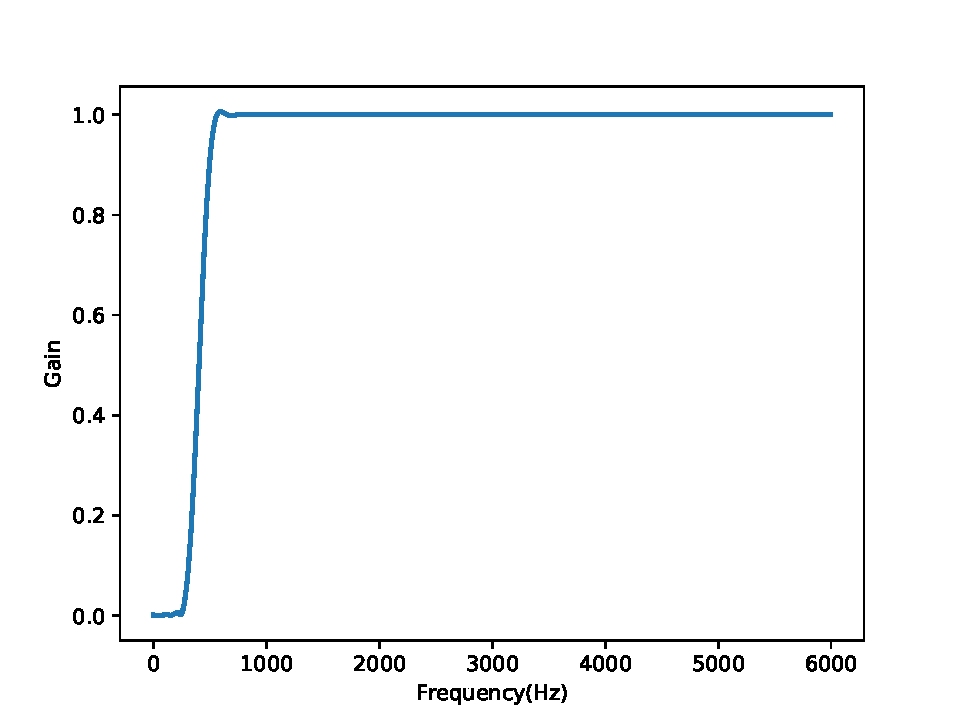
\includegraphics[width=1\linewidth]{img/thd_hpf_resp.pdf}
		\caption{}
		\label{fig:opq:8:1}
	\end{subfigure}%
	\begin{subfigure}{.5\textwidth}
		\centering
		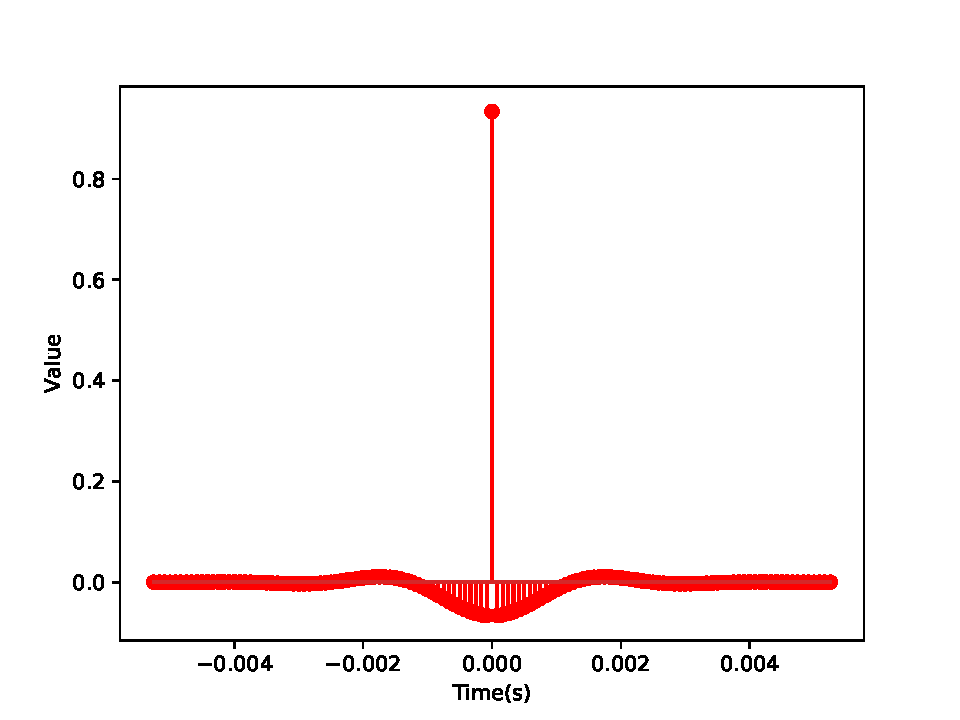
\includegraphics[width=1\linewidth]{img/thd_hpf.pdf}
		\caption{}
		\label{fig:opq:8:2}
	\end{subfigure}

	\begin{subfigure}{.5\textwidth}
		\centering
		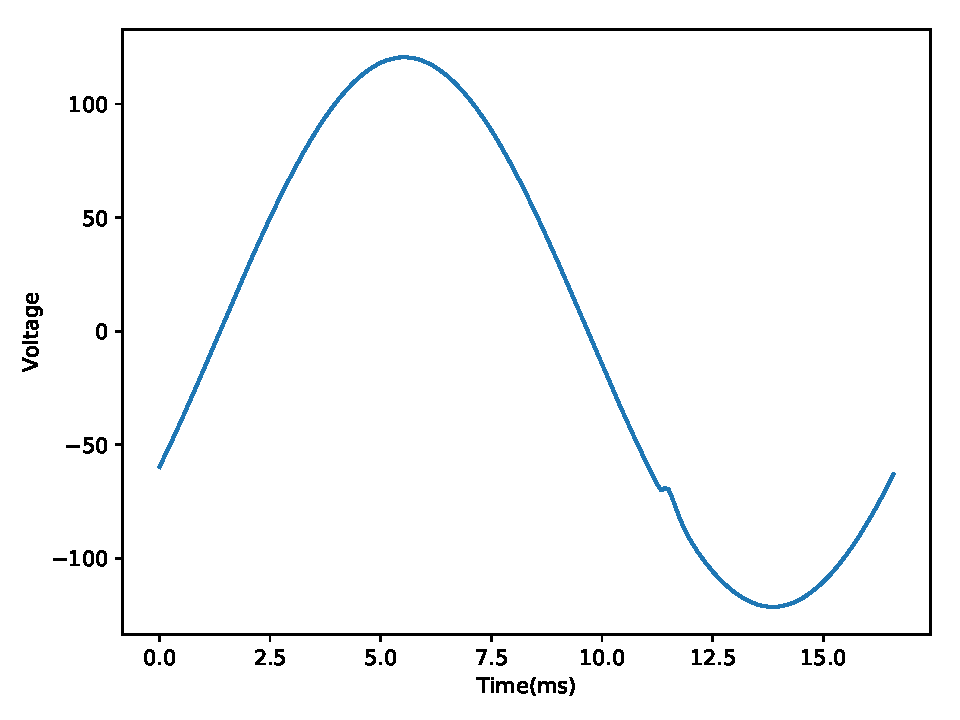
\includegraphics[width=0.86\linewidth]{img/box_eval/5v_transient.pdf}
		\caption{}
		\label{fig:opq:8:3}
	\end{subfigure}%
	\begin{subfigure}{.5\textwidth}
		\centering
		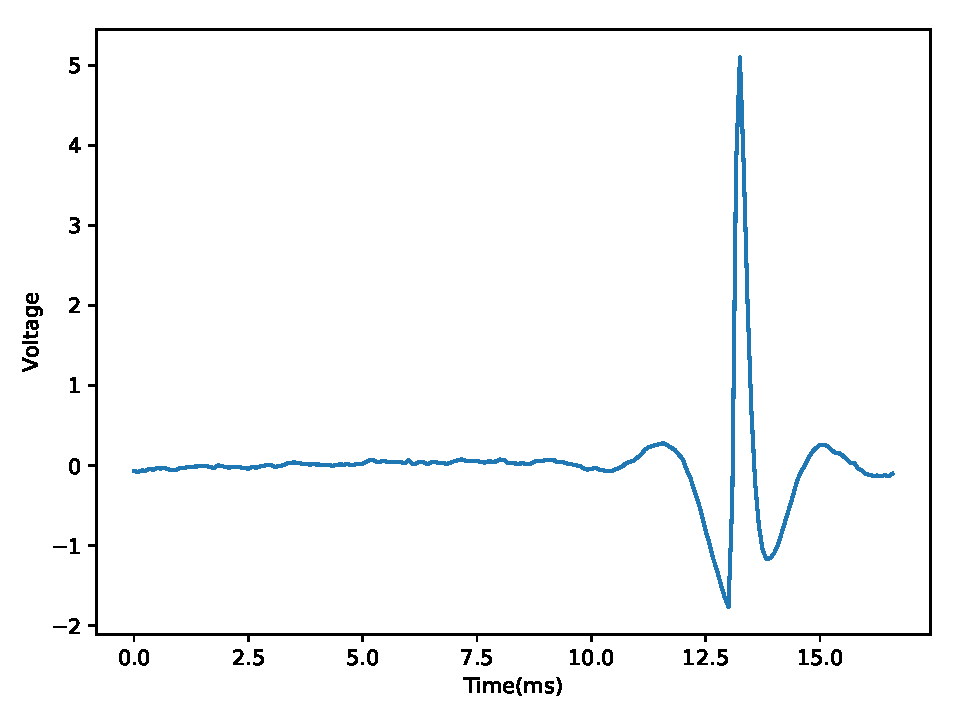
\includegraphics[width=0.86\linewidth]{img/box_eval/5v_transient_filtered.pdf}
		\caption{}
		\label{fig:opq:8:4}
	\end{subfigure}
	\caption{THD detection filtering. (a) Filter gain. (b) Filter response. (c) A 5V transient superimposed onto a fundamental. (d) Filter result from (c).}
	\label{fig:opq:8}
\end{figure}

It should be noted, that this transient detection method is susceptible to THD fluctuations, since any harmonic above $400Hz$ will remain in the filtered waveform.
However, since the THD information is transmitted along with the transient detection metric, they can be correlated in downstream transient detection.
This effect can be seen in Figure~\ref{fig:opq:9}.
This figure shows both the THD and transient detection metric during a transient event.
A small transient of approximately 1.6V was observed occurring at 2600s, while the sensitivity of the transient metric is clearly visible, particularly between 3000s and 4500s.

\begin{figure}[h]
	\begin{center}
		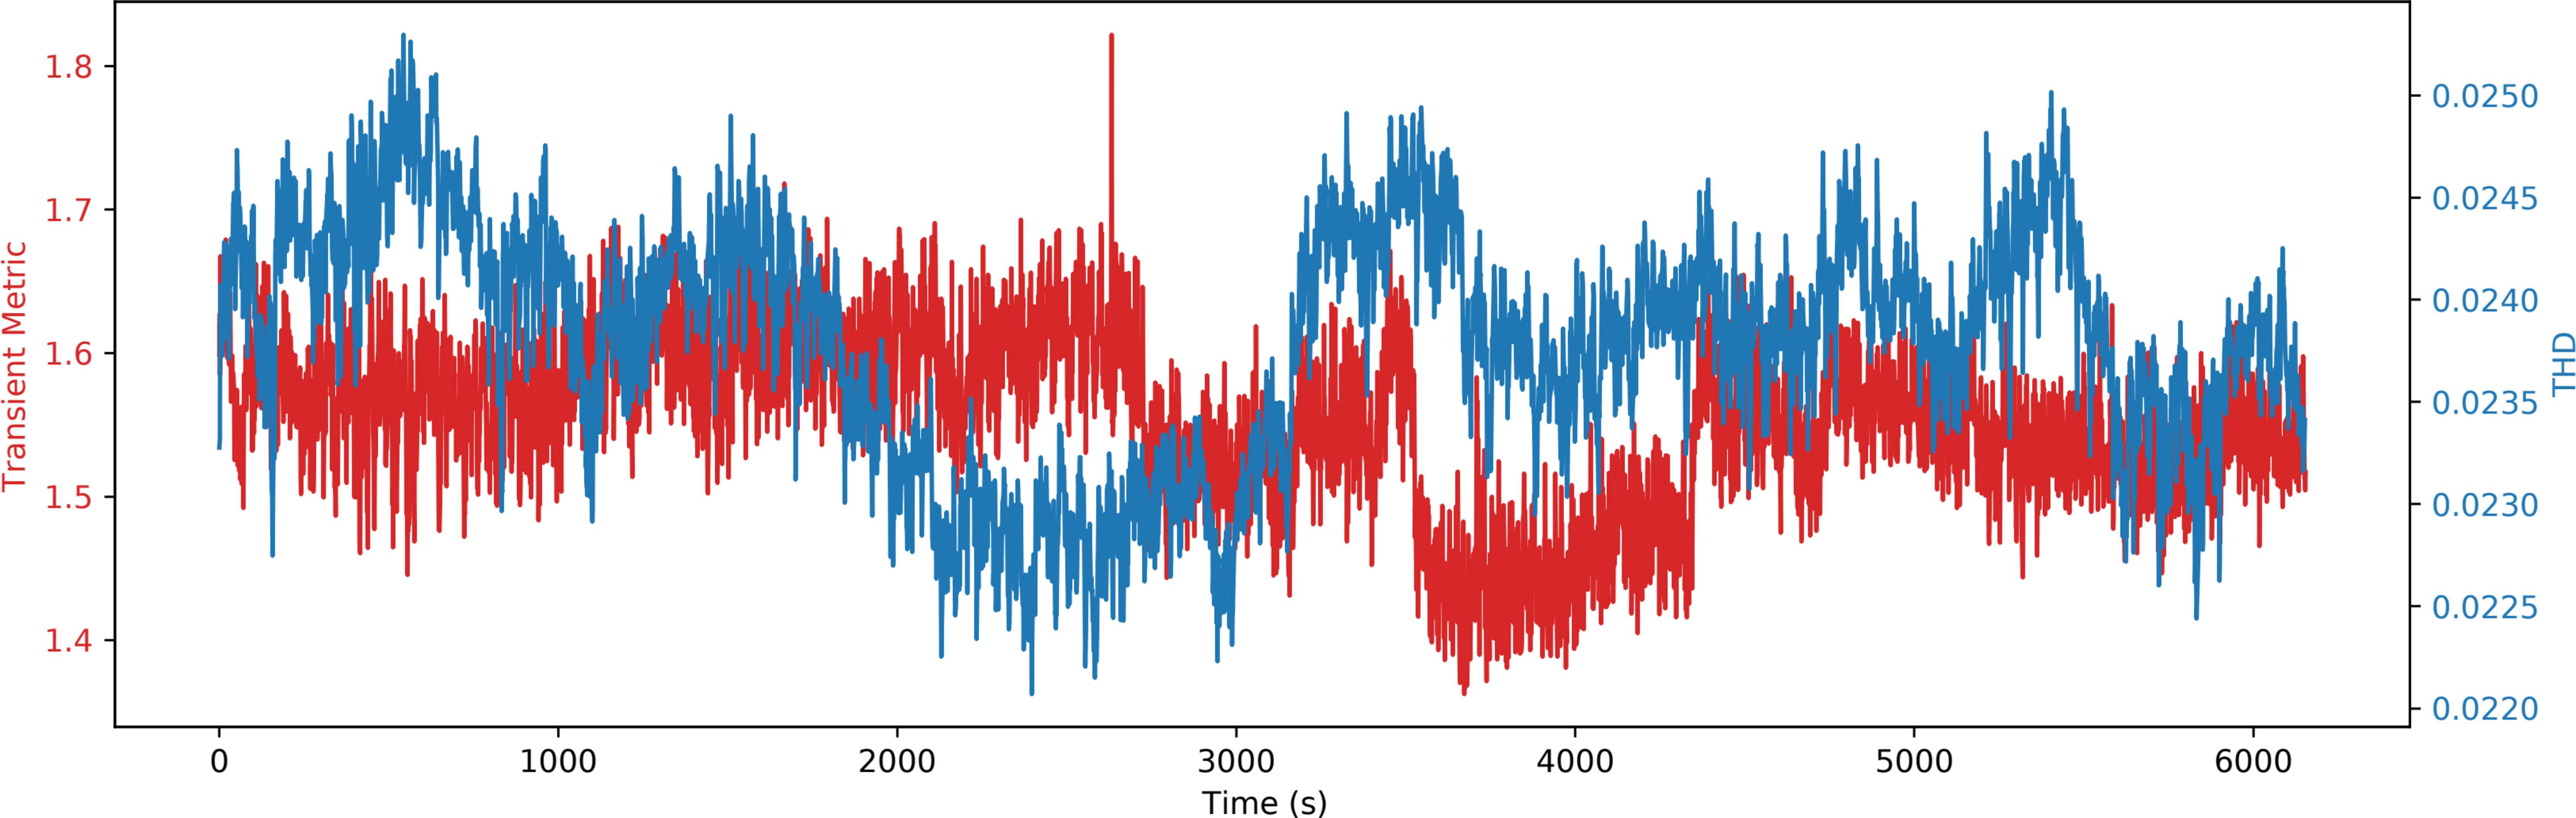
\includegraphics[width=1\textwidth]{img/trans_thd_det.pdf}
	\end{center}
	\caption{THD and Transient detection metric.}
	\label{fig:opq:9}
\end{figure}

\subsection{Network Communication}\label{subsec:network-communication}

Computed fundamental frequency and $V_{rms}$ are transmitted to the Makai service for aggregation.
Data transmission is handled using ZeroMq software stack with Curve25519 elliptic curve encryption.
Each device holds a unique private and public key, as well as the servers public key, allowing both the Makai service and the OPQ Box 2 to verify it's peer.
Internally metrics transmission uses ZeroMq's PUB/SUB protocol.
This protocol is a publish subscribe topology, with each message containing the topic, and a payload.
Additionally ZeroMq pub-sub topology allows for multiple sub peers with subscriptions forwarder to the publisher automatically via a side channel.
This allows for the aggregation service to be spread across multiple nodes, with minimal network overhead.

If the aggregation service determines that an anomaly has occurred, it is able to request raw waveform from the OPQ Box 2 RDRB via a separate ZeroMq pub sub channel.
If the RDRB buffer contains data for the requested temporal range, OPQ Box 2 transmits the available data to the aggregation service via a push pull ZeroMq channel.
Protobuf message serialization is used to encode messages across the OPQ ecosystem.


In order to make a distributed measurement, all of the OPQ Boxes on the OPQ network need to maintain an accurate time reference.
Time synchronization across multiple OPQ Boxes is accomplished using the Network Time Protocol.
The expansion port of the OPQ Box 2 supports a GPS receiver.
GPS receivers require line of sight to the sky, and since the with out on-board real-time clock, every power interruption requires a GPS cold start.
NTP performance has been verified against GPS resulting in time error of $8ms\pm 5ms$ which is typical for NTP running over the Internet with a close by NTP server.
This error is visualized in a Figure~\ref{fig:opq:6:2}.
With a large coincidental $V_{pp}$ drop across two devices, a 7ms phase error is clearly visible.


\section{OPQ Makai}\label{sec:opq-makai}

OPQ Makai implements the Napali Framework requirements for a ``sink''.
 It is a distributed extensible microservice framework responsible for receiving the triggering stream from the OPQ Boxes, locating anomalous temporal regions and requesting raw waveform for the anomalous time ranges.
 As evident from the block diagram shown in Figure~\ref{fig:opq:10}, Makai consists of four major components: Acquisition Broker, Triggering Broker, Event Service and the Acquisition Service.
\begin{figure}[h]
  \begin{center}
  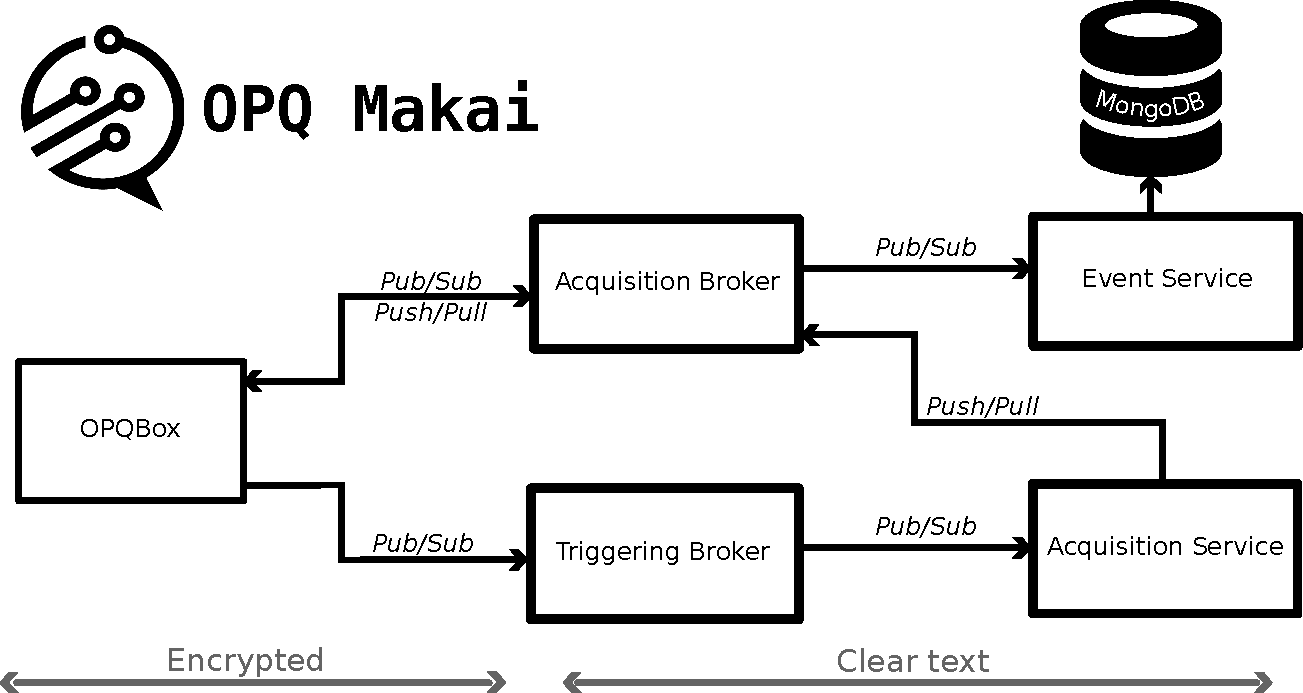
\includegraphics[width=0.7\textwidth]{img/makai_main.pdf}
  \end{center}
  \caption{Block diagram of the OPQ Makai.}
  \label{fig:opq:10}
\end{figure}

\subsection{Triggering Broker}\label{subsec:triggering-broker}

The triggering Broker is perhaps the simplest component of the OPQ Makai system.
The triggering stream generated by the OPQ Boxes is encrypted to preserve users privacy.
In order to minimize the CPU time spent decrypting the data across multiple OPQ services, the Triggering Broker is used to decrypt the data and send clear text measurements across the rest of the OPQ ecosystem.
Triggering Broker uses the ZeroMq subscribe socket to receive data form OPQ Boxes, and sends it via a publish socket to any connected client.
Each publish message is published to a topic which corresponds to the ASCII representation of the originating OPQ Box ID.
This allows services which utilize the Triggering broker to select a subset of IDs to operate on.
This is useful for load balancing the backend services, or dividing the OPQ network into separate regions with no electrical connections between them.

OPQ Box transmits metrics which make up the triggering stream in form of Protobuf encoded messages.
The structure of triggering messages is shown in Table \ref{tbl:opq:trg_struct}.
\begin{center}
	\begin{table}[!ht]
		\caption{Triggering message structure.}
		\label{tbl:opq:trg_struct}
		\begin{tabularx}{\textwidth}[t]{ssb}
			\arrayrulecolor{green}\hline
			\textbf{\textcolor{myGreen}{Triggering Message}} & &\\
			\hline
			\textbf{Field} & \textbf{Type} & \textbf{Description} \\
			\arrayrulecolor{black}\hline
			\textbf{box\_id} & \textit{uint32} & Device ID this message originated from.\\
			\arrayrulecolor{black}\hline
			\textbf{timestamp\_ms} & \textit{uint64} & Timestamp corresponding to the first cycle in the temporal window.\\
			\arrayrulecolor{black}\hline
			\textbf{metrics} & \textit{map$<$string, Metric$>$} & A map of metric names to corresponding values.\\
			& & \\
			\arrayrulecolor{green}\hline
			\textbf{\textcolor{myGreen}{Metric}} & &\\
			\hline
			\textbf{Field} & \textbf{Type} & \textbf{Description} \\
			\arrayrulecolor{black}\hline
			\textbf{min} & \textit{f32} & Minimum observed in this window.\\
			\arrayrulecolor{black}\hline
			\textbf{max} & \textit{f32} & Maximum observed in this window.\\
			\arrayrulecolor{black}\hline
			\textbf{average} & \textit{f32} & Average observed in this window.\\
		\end{tabularx}
	\end{table}
\end{center}


\subsection{Acquisition Broker}\label{subsec:acquisition-broker}

The Acquisiton Broker manages the two-way communication between the OPQ Boxes and the rest of the cloud infrastructure.
Unlike the triggering stream which originates from the OPQ Box, two way communication is always initiated by the cloud services.
Two way communication is realized via a command response interface, where the OPQ service initiates the communication by sending a clear text command to the Acquisition Broker, which then forwards it in the encrypted form to the appropriate OPQ Boxes.

As mention in the OPQ Box section, all communication between the OPQ Box and Makai is serialized using Google Protobuf.
Protobuf allows for polylingual communication between software components across network boundaries.
This is particularly important in case of the Acquisition and Triggering brokers, since they facilitate all inter-network communication.
All commands between services downstream of the Acquisition Broker and OPQ Boxes take on the form shown in Table \ref{tbl:opq:cmd_struct}.

\begin{center}
	\begin{table}[!ht]
		\caption{Command/Response message structure.}
		\label{tbl:opq:cmd_struct}
		\begin{tabularx}{\textwidth}[t]{ssb}

			\arrayrulecolor{green}\hline
			\textbf{\textcolor{myGreen}{Makai $\rightarrow$ OPQ Box}} & &\\
			\hline
			\textbf{Field} & \textbf{Type} & \textbf{Description} \\
			\arrayrulecolor{black}\hline
			\textbf{seq} & \textit{uint32} & Sequence number for the command.\\
			\arrayrulecolor{black}\hline
			\textbf{box\_id} & \textit{uint32} & Device ID this command will be routed to.\\
			\arrayrulecolor{black}\hline
			\textbf{timestamp\_ms} & \textit{uint64} & Millisecond timestamp, created on command issue.\\
			\arrayrulecolor{black}\hline
			\textbf{identity} & \textit{string} & Identity of the sender.\\
			\arrayrulecolor{black}\hline
			\textbf{command} & \textit{Command} & Command payload.\\
			& &\\
			\arrayrulecolor{green}\hline
			\textbf{\textcolor{myGreen}{OPB Box $\rightarrow$ Makai}} & &\\
			\hline
			\textbf{Field} & \textbf{Type} & \textbf{Description} \\
			\arrayrulecolor{black}\hline
			\textbf{box\_id}  & \textit{uint32} & Device ID this command is routed from.\\
			\arrayrulecolor{black}\hline
			\textbf{seq} & \textit{uint32} & Sequence number of the response\\
			\arrayrulecolor{black}\hline
			\textbf{timestamp\_ms} & \textit{uint64} & Millisecond timestamp, created on response issue.\\
			\arrayrulecolor{black}\hline
			\textbf{response} & \textit{Response} & Response payload.\\
		\end{tabularx}
	\end{table}
\end{center}

In order to send a message to an OPQ Box, a client generates a \textbf{Makai $\rightarrow$ OPQ Box} command containing its identity, serializes it, and forwards it to the Acquisition broker's push port.
The acquisition broker assigns a unique sequence number to the request and stores it in an internal synchronized key value store along with the sender identity.
The message is re-serialized and sent out to the desired OPQ Box via the broker's encrypted pub interface.
Each message sent to the OPQ Box generates a response in form of \textbf{OPB Box $\rightarrow$ Makai} message.
This response is received by the Acquisition broker via encrypted pull interface, deserialized and validated.
Response sequence number is used to determine the recipient's identity, and the message is forwarded to the correct recipient via the broker's cleartext publish interface.
It is important to note that the service which generates a command and the service which receives the response need not be the same, and a command originator may place the box response into the subscribe stream of a different service.
This detail becomes important during the discussion of the Event service.
Furthermore, sending and receiving messages occurs asynchronously, thus multiple clients can communicate with multiple Boxes at the same time.
Finally, a garbage collector cleans the synchronised key value store every hour, removing sequence numbers which did not receive a response for an OPQ Box.
These sequence numbers and identities are logged, since a lack of a response indicates a device or a network fault, or a buggy client.

There are four unique payload commands/responses which an OPQ Box understands.
These payloads are ignored by the Acquisition Broker and are simply forwarded to the recipient.
Bellow is the list of commands/responses:
\begin{itemize}
	\item{\textbf{(HEALTH) Health:}} The health command is broadcast periodically across all of the OPQ Boxes, in order to collect diagnostics from all OPQ devices.
	The OPQ Box response to this command contains diagnostic information, such as the timestamp of the last event requested, ip address and the name and strength of the WIFI network the OPQ Box is connected to.
	\item{\textbf{(CMW) Change measurement window:}} This command allows downstream services to vary how often a triggering stream message is generated and delivered to the triggering broker.
	This is accomplished by varying the length of the temporal window used to derive the triggering metrics.
	\item{\textbf{(RD) Send raw data:}} This command instructs the OPQ Box to send data from the its raw data buffer to the cloud.
	\item {\textbf{(PLG) Plugin:}} Send a binary payload directly to a OPQ Box Plugin.
\end{itemize}
Data fields for each command are described in the Tables \ref{tbl:opq:cmd_payload} and \ref{tbl:opq:rsp_payload}.
Notice that an \textbf{Err} response does not correspond to any commands described above.
OPQBox generates this response under following conditions:
\begin{itemize}
	\item Command payload could not be parsed.
	\item $start\_ms > end\_ms$ in case of the RD command.
	\item box\_id field does not match the destination OPQ Box.
	\item PLG command is attempting to route to a OPQ Box plugin that is not loaded by the recipient.
\end{itemize}
In the current implementation, OPQ Makai protocol does not support multicast addressing of OPQ Boxes.
Furthermore, due to the limitations of the ZeroMq API, there is no stable method of querying the clients connected to a particular port.
Utilities which query all available devices, such as a periodic health check service, query the MongoDB database for a list of devices registered to the OPQ network, and send their queries to each box individually.
\begin{center}
	\begin{table}[!ht]
		\caption{Command Payloads}
		\label{tbl:opq:cmd_payload}
		\begin{tabularx}{\textwidth}[t]{ssb}

			\arrayrulecolor{green}\hline
			\textbf{\textcolor{myGreen}{HEALTH}} & &\\
			\hline
			N/A & & This command has no fields.\\
			& &\\
			\arrayrulecolor{green}\hline
			\textbf{\textcolor{myGreen}{CMW}} & &\\
			\hline
			\textbf{Field} & \textbf{Type} & \textbf{Description} \\
			\arrayrulecolor{black}\hline
			\textbf{measurement\_rate}  & \textit{uint32} & Number of cycles per triggering triggering message.\\
			& &\\
			\arrayrulecolor{green}\hline
			\textbf{\textcolor{myGreen}{RD}} & &\\
			\hline
			\textbf{Field} & \textbf{Type} & \textbf{Description} \\
			\arrayrulecolor{black}\hline
			\textbf{start\_ms} & \textit{uint64} & Timestamp defining the beginning of the region of interest.\\
			\arrayrulecolor{black}\hline
			\textbf{end\_ms} & \textit{uint64} & Timestamp defining the end of the region of interest.\\
			\arrayrulecolor{black}\hline
			\textbf{wait} & \textit{bool} & A flag indicating that a Box must wait if \textbf{end\_ms} is in the future.\\
			& & \\
			\arrayrulecolor{green}\hline
			\textbf{\textcolor{myGreen}{PLG}} & &\\
			\hline
			\textbf{Field} & \textbf{Type} & \textbf{Description} \\
			\arrayrulecolor{black}\hline
			\textbf{plugin\_name} & \textit{string} & Name of the plugin.\\
			\arrayrulecolor{black}\hline
			\textbf{message} & \textit{bytes} & Binary payload for the plugin.\\

		\end{tabularx}
	\end{table}
\end{center}

\begin{center}
	\begin{table}[!ht]
		\caption{Response Payloads}
		\label{tbl:opq:rsp_payload}
		\begin{tabularx}{\textwidth}[t]{ssb}

			\arrayrulecolor{green}\hline
			\textbf{\textcolor{myGreen}{HEALTH}} & &\\
			\hline
			\textbf{Field} & \textbf{Type} & \textbf{Description} \\
			\arrayrulecolor{black}\hline
			\textbf{mac\_addr} & \textit{string} & Mac address of the box.\\
			\arrayrulecolor{black}\hline
			\textbf{wifi\_network} & \textit{string} & SSID of connected Wifi network.\\
			\arrayrulecolor{black}\hline
			\textbf{ip} & \textit{string} & Ip address of the wlan0 interface.\\
			\arrayrulecolor{black}\hline
			\textbf{uptime} & \textit{uint64} & Device uptime in ms.\\
			\arrayrulecolor{black}\hline
			\textbf{calibration\_constant} & \textit{f32} & Calibration constant for the device.\\
			\arrayrulecolor{black}\hline
			\textbf{pub\_key} & \textit{string} & Byte64 encoded public key of the device.\\
			\arrayrulecolor{black}\hline
			\textbf{measurement\_rate} & \textit{string} & How often a triggering message is produced.\\

			& &\\
			\arrayrulecolor{green}\hline
			\textbf{\textcolor{myGreen}{CMW}} & &\\
			\hline
			\textbf{Field} & \textbf{Type} & \textbf{Description} \\
			\arrayrulecolor{black}\hline
			\textbf{measurement\_rate}  & \textit{uint32} & Old measurement rate.\\
			& &\\
			\arrayrulecolor{green}\hline
			\textbf{\textcolor{myGreen}{RD}} & &\\
			\hline
			\textbf{Field} & \textbf{Type} & \textbf{Description} \\
			\arrayrulecolor{black}\hline
			\textbf{start\_ms} & \textit{uint64} & Timestamp defining the beginning of the region of interest.\\
			\arrayrulecolor{black}\hline
			\textbf{end\_ms} & \textit{uint64} & Timestamp defining the end of the region of interest.\\
			\arrayrulecolor{black}\hline
			\textbf{data} & \textit{Cycle[..]} & Data divided into single cycle windows structures. \\
			& & \\
			\arrayrulecolor{green}\hline
			\textbf{\textcolor{myGreen}{Cycle}} & &\\
			\hline
			\textbf{Field} & \textbf{Type} & \textbf{Description} \\
			\arrayrulecolor{black}\hline
			\textbf{datapoints} & \textit{int16[200]} & Raw ADC samples for one cycle window.\\
			\arrayrulecolor{black}\hline
			\textbf{timestamp\_ms} & \textit{uint64} & Timestamp of the last sample.\\
			& & \\
			\arrayrulecolor{green}\hline
			\textbf{\textcolor{myGreen}{PLG}} & &\\
			\hline
			\textbf{Field} & \textbf{Type} & \textbf{Description} \\
			\arrayrulecolor{black}\hline
			\textbf{OK} & \textit{bool} & Flag indicating that the command was successfully routed to a plugin.\\
			& & \\
			\arrayrulecolor{green}\hline
			\textbf{\textcolor{myGreen}{Err}} & &\\
			\hline
			\textbf{Field} & \textbf{Type} & \textbf{Description} \\
			\arrayrulecolor{black}\hline
			\textbf{code} & \textit{uint32} & Error Code.\\
			\arrayrulecolor{black}\hline
			\textbf{Error} & \textit{string} & Human readable error string.\\
		\end{tabularx}
	\end{table}
\end{center}

\subsection{Acquisition Service}\label{subsec:acquisition-service}

The Acquisition Service middleware resides between the Triggering and Acquisition Brokers.
The Acquisition Service is responsible for the following tasks:
\begin{enumerate}
	\item Computation of statistics of the incoming triggering stream.
	\item Hosting plugins for triggering stream analysis.
	\item Generating data event requests for OPQ Boxes.
\end{enumerate}
A block diagram of the Acquisition Service is shown in Figure \ref{fig:opq:makai_aqs}.
\begin{figure}[h]
	\begin{center}
		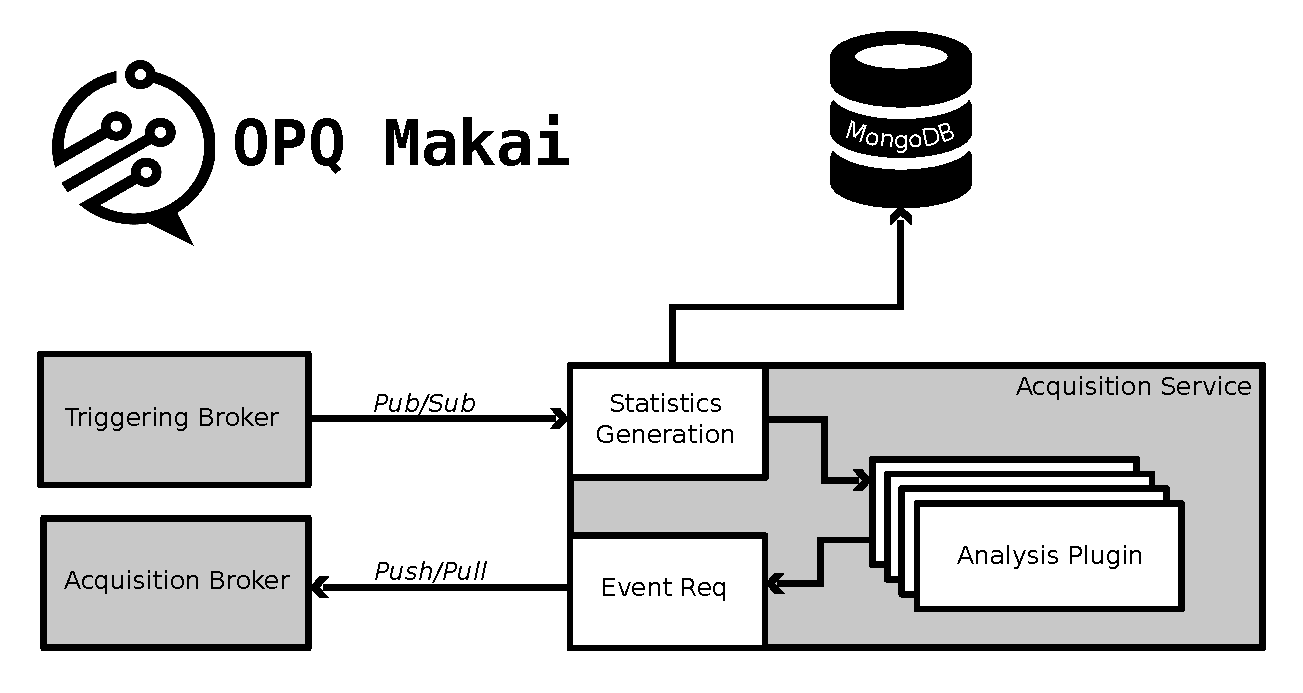
\includegraphics[width=0.6\textwidth]{img/makai_aqs.pdf}
	\end{center}
	\caption{Block diagram of the Acquisition Service.}
	\label{fig:opq:makai_aqs}
\end{figure}

\subsubsection{Triggering Stream Statistics.}

The Acquisition Service accesses the triggering stream by connecting to the publish socket of the Triggering broker.
Since the connection is managed through the ZeroMq publish-subscribe socket, several Acquisition Services can be connected to a single Triggering broker endpoint each servicing a subset of OPQ Boxes by subscribing to only specific devices.
This functionality is used to manage devices that the OPQ project sends to the mainland for evaluation by organisations interested in the project.
These loner devices participate in their own triggering schemes, and do not contaminate the triggering stream with messages about an unconnected grid.

Triggering messages received by the Acquisition service are buffered and stored in the MongoDB database.
There are two types of statistics accumulated by the Acquisition Service:
\begin{enumerate}
	\item \textit{Measurements:} Every triggering stream message gets converted to a set measurement.
	\item \textit{Trends:} One minute window of triggering stream messages get feature extracted and stored.
\end{enumerate}

Measurements have a one-to-one relationship with a triggering messages and take form of MongoDB documents described in Table \ref{tbl:opq:measurement_db}.
Measurement documents have an expire\_at field instructing MongoDB to clean up the measurement collection after after a predetermined time period.
Currently measurement documents persist for 24 hours.
\begin{center}
	\begin{table}[!ht]
		\caption{Measurement Document.}
		\label{tbl:opq:measurement_db}
		\begin{tabularx}{\textwidth}[t]{ssb}
			\textbf{Field} & \textbf{Type} & \textbf{Description} \\
			\arrayrulecolor{black}\hline
			\textbf{box\_id} & \textit{string} & OPQ Box ID.\\
			\arrayrulecolor{black}\hline
			\textbf{timestamp\_ms} & \textit{uint64} & Millisecond timestamp.\\
			\arrayrulecolor{black}\hline
			\textbf{voltage} & \textit{f32} & $V_{rms}$ average value.\\
			\arrayrulecolor{black}\hline
			\textbf{thd} & \textit{f32} & THD average value\\
			\arrayrulecolor{black}\hline
			\textbf{frequency} & \textit{f32} & Frequency average value\\
			\arrayrulecolor{black}\hline
			\textbf{expire\_at} & \textit{f32} & Deletion time for the measurement.\\
		\end{tabularx}
	\end{table}
\end{center}

Trends consist of feature extracted statistics accumulated from 1 minute of triggering measurements.
The statistics computed are minimum, maximum and average for each box metric.
Similarly to the Measurement documents, Trend documents expire after a predetermined period of time.
Currently trends are retained for 7 days.
Structure of a Trend document is shown in Table \ref{tbl:opq:trend_db}.

\begin{center}
	\begin{table}[!ht]
		\caption{Trend Document.}
		\label{tbl:opq:trend_db}
		\begin{tabularx}{\textwidth}[t]{ssb}
			\arrayrulecolor{green}\hline
			\textbf{\textcolor{myGreen}{Trend Document}} & &\\
			\hline
			\textbf{Field} & \textbf{Type} & \textbf{Description} \\
			\arrayrulecolor{black}\hline
			\textbf{box\_id} & \textit{string} & OPQ Box ID.\\
			\arrayrulecolor{black}\hline
			\textbf{timestamp\_ms} & \textit{uint64} & Millisecond timestamp.\\
			\arrayrulecolor{black}\hline
			\textbf{voltage} & \textit{Statistics} & $V_{rms}$ average value.\\
			\arrayrulecolor{black}\hline
			\textbf{thd} & \textit{Statistics} & THD average value\\
			\arrayrulecolor{black}\hline
			\textbf{frequency} & \textit{Statistics} & Frequency average value\\
			\arrayrulecolor{black}\hline
			\textbf{expire\_at} & \textit{u64} & Deletion time for the measurement.\\
			& & \\
			\arrayrulecolor{green}\hline
			\textbf{\textcolor{myGreen}{Statistics}} & &\\
			\hline
			\textbf{Field} & \textbf{Type} & \textbf{Description} \\
			\arrayrulecolor{black}\hline
			\textbf{Min} & \textit{f32} & Minimum observed during the trend window.\\
			\arrayrulecolor{black}\hline
			\textbf{Max} & \textit{f32} & Maximum observed during the trend window.\\
			\arrayrulecolor{black}\hline
			\textbf{Average} & \textit{f32} & Average computed over the trend window.\\
			\arrayrulecolor{black}\hline
		\end{tabularx}
	\end{table}
\end{center}

\subsubsection{Triggering Analysis infrastructure.}

The Acquisition Service does not include any analysis capabilities by default.
Instead analysis is performed by shared library loadable plugins.
These plugins can be loaded and unloaded at runtime, thus allowing live upgrading and testing of new analysis methods.
Plugin are loaded using libdl by searching for C function hooks which produce a Rust structure which implements a plugin interface.
The interface as well as the prototype C hook function are shown below:

\begin{lstlisting}[language=Rust, style=colouredRust]
pub trait MakaiPlugin: Any {
  fn name(&self) -> &'static str;
  fn process_measurement(&mut self, msg: Arc<Measurement>)->Option<Vec<Command>>;
  fn on_plugin_load(&mut self, json: String);
  fn on_plugin_unload(&mut self);
}
#[no_mangle]
pub extern "C" fn _plugin_create() -> *mut MakaiPlugin;

#[no_mangle]
pub extern "C" fn _plugin_destroy(plg : *mut MakaiPlugin);
\end{lstlisting}

The $\_plugin\_create$ function is marked as $no\_mangle$ which instructs the compiler to retain the function name so it can be located by the plugin loader.
It returns a mutable pointer to a boxed type which implements the MakaiPlugin interface.
Since Rust is a explicit memory management language, and the runtime is not aware of the internal structure of the Boxed type beyond its interface,
a helper function $\_plugin\_destroy$ is used to cleanup the plugin object during the unloading process.
Each plugin runs in a separate thread with a synchronized queue from which it draws measurement messages.
If a plugins is not able to keep up with the triggering stream, The Acquisition service will start dropping messages from its input queue,
and a message indicating this fault will be stored in its log.
Once a plugin is loaded it will receive its settings in the form of a JSON encoded string using the $on\_plugin\_load$ method.
This allows it to initialize all of the internal data structures to a known state.
Similarly $on\_plugin\_unload$ method is used to inform the plugin that it will be immanently unloaded.

The processing of the triggering stream occurs in the $process\_measurement$ method.
This methods takes a reference counted Measurement message in form shown in Table \ref{tbl:opq:trg_struct}.
Return type of this method is an optional list of commands to forward to the Acquisition broker in form shown in Table \ref{tbl:opq:cmd_struct}.
All of the Commands in the list are treated to be pertaining to the same event.

\subsubsection{Event Request.}
Once a plugin determines that an event of interest has taken place, it will emit a list of \textbf{RD} commands with structure shown in Table \ref{tbl:opq:cmd_payload}.
Event requester will fill in the identity field with the following string:
\[ identity = ``data\_" + EVENT\_TOKEN +"\_" + ACQ\_UUID\]

The ``$data\_$" prefix is used to route the messages responses from the OPQ Box to the Event storage service.
As mentioned previously, responses from device command need not return to the same service that sent the command.
Instead, the responses will be routed to a service which is subscribed to the identity used in the request.
The $EVENT\_TOKEN$ root is a 16 character random hexadecimal string, which identifies data request corresponding to the same event event.
Since a single event may contain data from multiple OPQ Boxes, and each event will have a unique $EVENT\_TOKEN$ root.
The $ACQ\_UUID$ postfix is used to identify the Acquisition service which triggered the data request.
Multiple Acquisition Services can be used to service the OPQ network, and each one is identified using it's own UUID identifier.
This identifier may be assigned to each service via the configuration file, or autogenerated at startup.
Once the identity of each command is filled in, each command is forwarded to the Acquisition broker for routing to the OPQ Box experiencing a power quality disturbance.

\subsection{Event Service.}\label{subsec:event-service}

The Event service is a microservice which stores raw data generated by OPQ Boxes in the MongoDB Database.
On initialization, the Event service queries MongoDB database for the highest event number recorded so far, connects to the Acquisition Broker's publish port,
and subscribes to all messages that start with the prefix ``$data\_$".
This allows the Event service to capture every response from OPQ Boxes generated from commands issued by the Acquisition service plugins.
Once the Event service receives a data response with an identity containing an $EVENT\_TOKEN$ it hasn't seen before it will increment the event number, and
store it in an internal key value store.
This way every future data message which contains that $EVENT\_TOKEN$, it will be appended to the same event.
ER diagram of the MongoDB event storage is shown in Figure \ref{fig:opq:mongo_er}.
The Events collection contains metadata for individual events.
Box\_events collection contains metadata for event information from individual OPQ devices.
Finally gridfs, MongoDB's internal file storage, is used for storing event data.

\begin{figure}[h]
	\begin{center}
		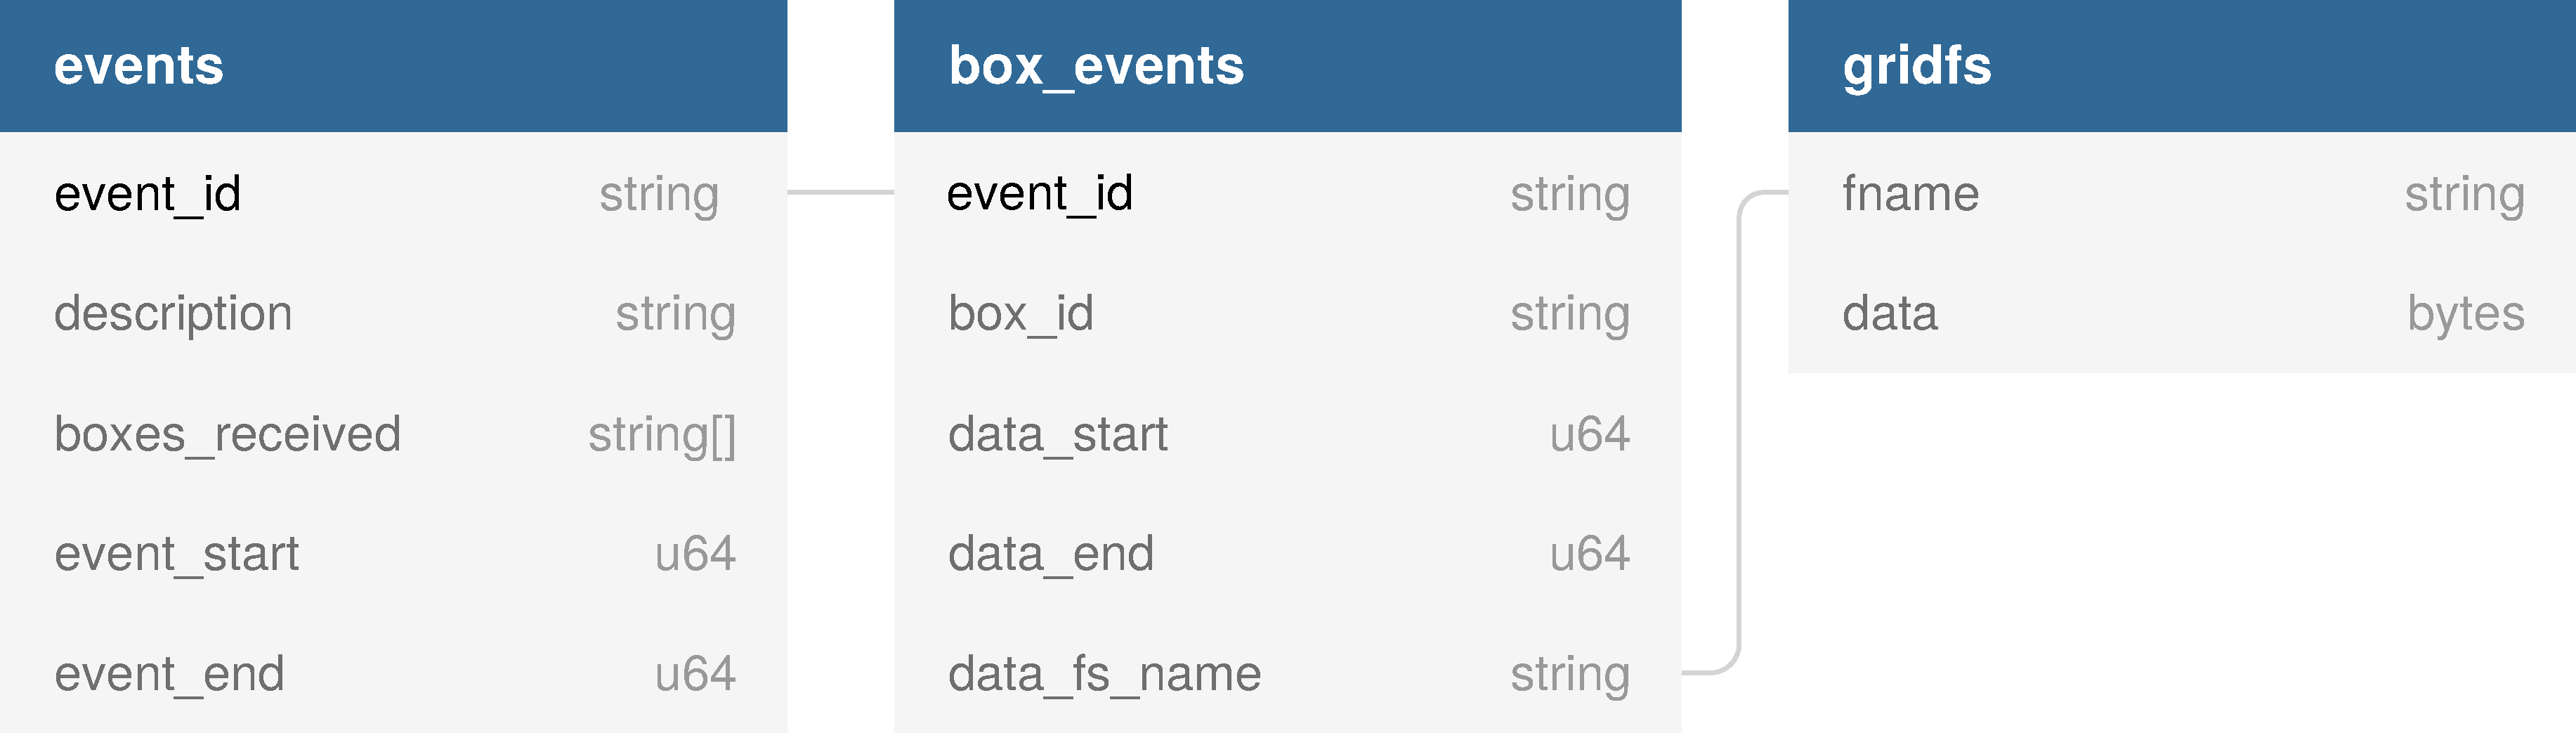
\includegraphics[width=0.9\textwidth]{img/mongo_event_storage.pdf}
	\end{center}
	\caption{ER diagram of event storage in MongoDB}
	\label{fig:opq:mongo_er}
\end{figure}

\subsection{Acquisition Service Plugins}\label{subsec:acquisition-service-plugins}

The Acquisition service plugins are responsible for monitoring the OPQ Box triggering streams and determining when to request raw data.
As such, the Acquisition service plugins constitute the majority of business logic for the OPQ Makai system.
There are currently four plugins developed for this system:
\begin{enumerate}
	\item Health Plugin.
	\item Debug Plugin.
	\item Threshold Trigger.
	\item Napali Trigger.
\end{enumerate}

\subsubsection{Health Plugin}

The health plugin is responsible for monitoring the triggering messages passing through the Acquisition Service.
It maintains a REST endpoint for reporting the OPQ Network status.
Furthermore the REST endpoint can be used to trigger a device for debugging purposes.

\subsubsection{Debug Plugin}
Debug plugin consists of a Lisp interpreter which can manipulate the triggering stream, and emit triggering commands for devices.
It can be used to quickly and interactively test new analysis methods, and debug the OPQ network.

\subsubsection{Threshold Trigger}
Threshold trigger plugin is used for in-situ comparison of a naive triggering method to Napali.
Every time the Threshold plugin receives a triggering message, it will check it against global thresholds.
If a metric value is outside of the predetermined thresholds the Triggering plugin will latch the timestamp and the id of the affected device.
Once the metric returns to normal, Threshold plugin will emit a request for raw data to the device which is experiencing an event.
If an event is longer then 50\% of the RDRB of an OPQ Box buffer an event will be broken up into several shorter events.
Threshold values for each metric are shown in Table \ref{tbl:opq:thresholds}

\begin{center}
	\begin{table}[!ht]
		\caption{Threshold values for each metric}
		\label{tbl:opq:thresholds}
		\begin{tabularx}{\textwidth}[t]{bss}
			\textbf{Metric} & \textbf{Min} &\textbf{Max}\\
			\arrayrulecolor{black}\hline
			$V_{rms}$ & $110V_{rms}$ & $130V_{rms}$ \\
			\arrayrulecolor{black}\hline
			$f_{fundamental}$ & $59.9Hz$ & $60.1Hz$ \\
			\arrayrulecolor{black}\hline
			$THD$ & N/A & $5\%$ \\
			\arrayrulecolor{black}\hline
			$Trans$ & N/A & $8V$ \\
		\end{tabularx}
	\end{table}
\end{center}

The Threshold Trigger plugin functions in the same way as a self-triggering device.
Since this method of event detection does not rely on intra-box information sharing, it functions in the same manner as if the OPQ Box itself
is performing event detection.
This allows for experimental comparison of the Napali method efficiency with the self-triggered methodology.

\subsubsection{Napali Trigger}\label{subsec:napali-trigger}

Napali Trigger plugin implements the Napali event detection method.
Napali Trigger state machine is kicked off the same way as the Threshold trigger.
If a received metric value is outside of the predetermined thresholds Napali plugin will latch the timestamp and the id of the affected device.
Similarly, once the offending metric from all devices return to normal, Napali plugin will emit a request for raw data to the device which is experiencing an event.
The main difference between the Napali trigger and the Threshold trigger are two-fold:
\begin{enumerate}
	\item An event is not considered finished until every device's metrics return to the nominal threshold range.
	\item Metric value is within the nominal threshold but outside 3 standard deviations of a mean, will cause a the device to be participating in the  event.
\end{enumerate}

The first difference allows Napali to track a propagation of a fault throughout the power delivery network.
Furthermore, during a lifetime of a power quality event, it may shift from one metric to another.
As the disturbance travels, through the power-grid, Napali will aggregate all of the temporally localized disturbances into one event.
The second disturbance allows for recording of sub-threshold data to be acquired from devices which did not pass the threshold, but exhibited anomalous behaviour.

The mean and standard deviation are calculated using two first order IIR filter loops as show in Equation \ref{eq:iir_mean}:
\begin{equation}\label{eq:iir_mean}
\begin{aligned}
	\mu_{n+1} = (1- \alpha)*\mu_{n} + \alpha * m \\
	\mu^2_{n+1} = (1- \alpha)*\mu^2_n + \alpha * m^2 \\
	\sigma^2_n = \mu^2_n - (\mu_n)^2 \\
	\sigma_n =\sqrt{\sigma_n^2}
\end{aligned}
\end{equation}
Where $\mu$ is the mean, $\sigma$ is the standard deviation, $m$ is the new sample and $\alpha$ is the decay parameter.
Notice that $(\mu)^2$ is the square of the mean, and $\mu^2$ is the mean of the squares.
The $\alpha$ parameter determines the memory of the filter, and can be computed as:
\begin{equation}\label{eq:iir_alpha}
\begin{aligned}
	\alpha = 1 - e^{2\pi\frac{T_{sample}}{T_{memory}}}
\end{aligned}
\end{equation}
Where $T_{sample}$ is the sampling rate of the system, 1s for OPQ, and $T_{memory}$ is the desired response of the system.

Using an IIR filter for mean and standard deviation calculation is computationally cheaper then using a FIR window.
Furthermore, using the IIR filter makes it trivial to tune the response of the system during runtime.

\section{OPQ Mauka}\label{sec:opq-mauka}
OPQ Mauka service is responsible for higher level classification and filtering of the anomalies generated by the OPQ Makai.
Since anomalies generation only
relies on the triggering stream features and not raw data, OPQ Makai is not able to ascertain if the anomaly is an actual power quality event, event type, or its severity.
OPQ Mauka on the other hand operates on the raw data, thus it is able to perform high level analysis to meet industry standards for vent classification.
The block diagram of the OPQ Mauka is shown in~\ref{fig:opq:11}.
\begin{figure}[h]
  \begin{center}
  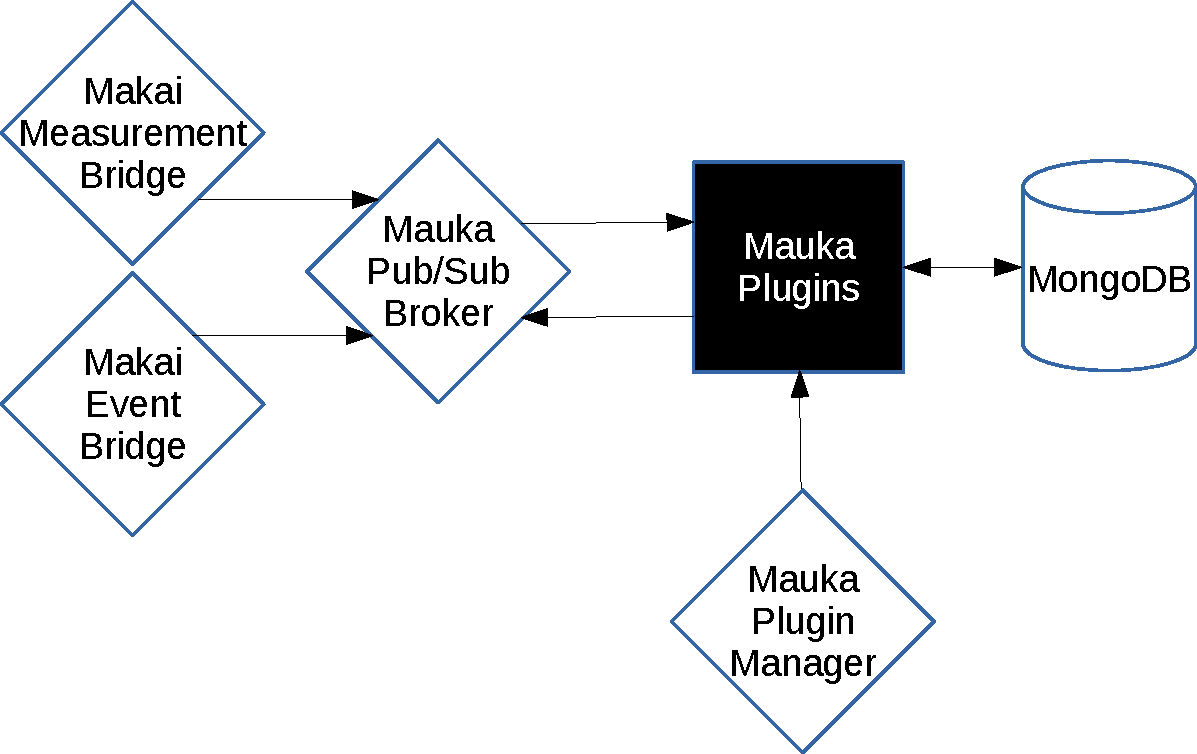
\includegraphics[width=0.6\textwidth]{img/mauka.pdf}
  \end{center}
  \caption{Block diagram of the OPQ Mauka.}
  \label{fig:opq:11}
\end{figure}

Currently OPQ Mauka supports the following classification strategies:
\begin{itemize}
	\item{\textbf{ITIC}} Power acceptability curve used to classify short term voltage sags.
	\item{\textbf{IEEE 1159 Voltage}} Voltage classification based on the IEEE 1159 power quality standard.
	\item{\textbf{Brownout Detection}} Classification of medium to long term voltage sags.
	\item{\textbf{Total Harmonic distortion}} Classification of events via harmonic analysis.
\end{itemize}

Once the anomaly is classified by OPQ Mauka, and the power quality characteristics are confirmed, it may be aggregated with other anomalies to form a disturbance.
Disturbances are composed of raw box data, analysis results as well as expert annotations and other metadata.

\section{OPQ View}\label{sec:opq-view}

OPQ View is the primary user interface to the OPQ ecosystem.
View is written in JavaScript using the Meteor framework, and provides a robust and easy to use interface to the OPQ Box triggering stream, Makai triggering anomalies, and to the Mauka PQ disturbances.
Furthermore, View provides an administration interface for initial setup and maintenance of the OPQ devices, and services.
Finally OPQ View monitors the health of the OPQ components, keeping track of the individual box uptimes, and component failures.
A screenshot of the recent OPQ View build is shown in Figure~\ref{fig:opq:12}

\begin{figure}[h]
  \begin{center}
  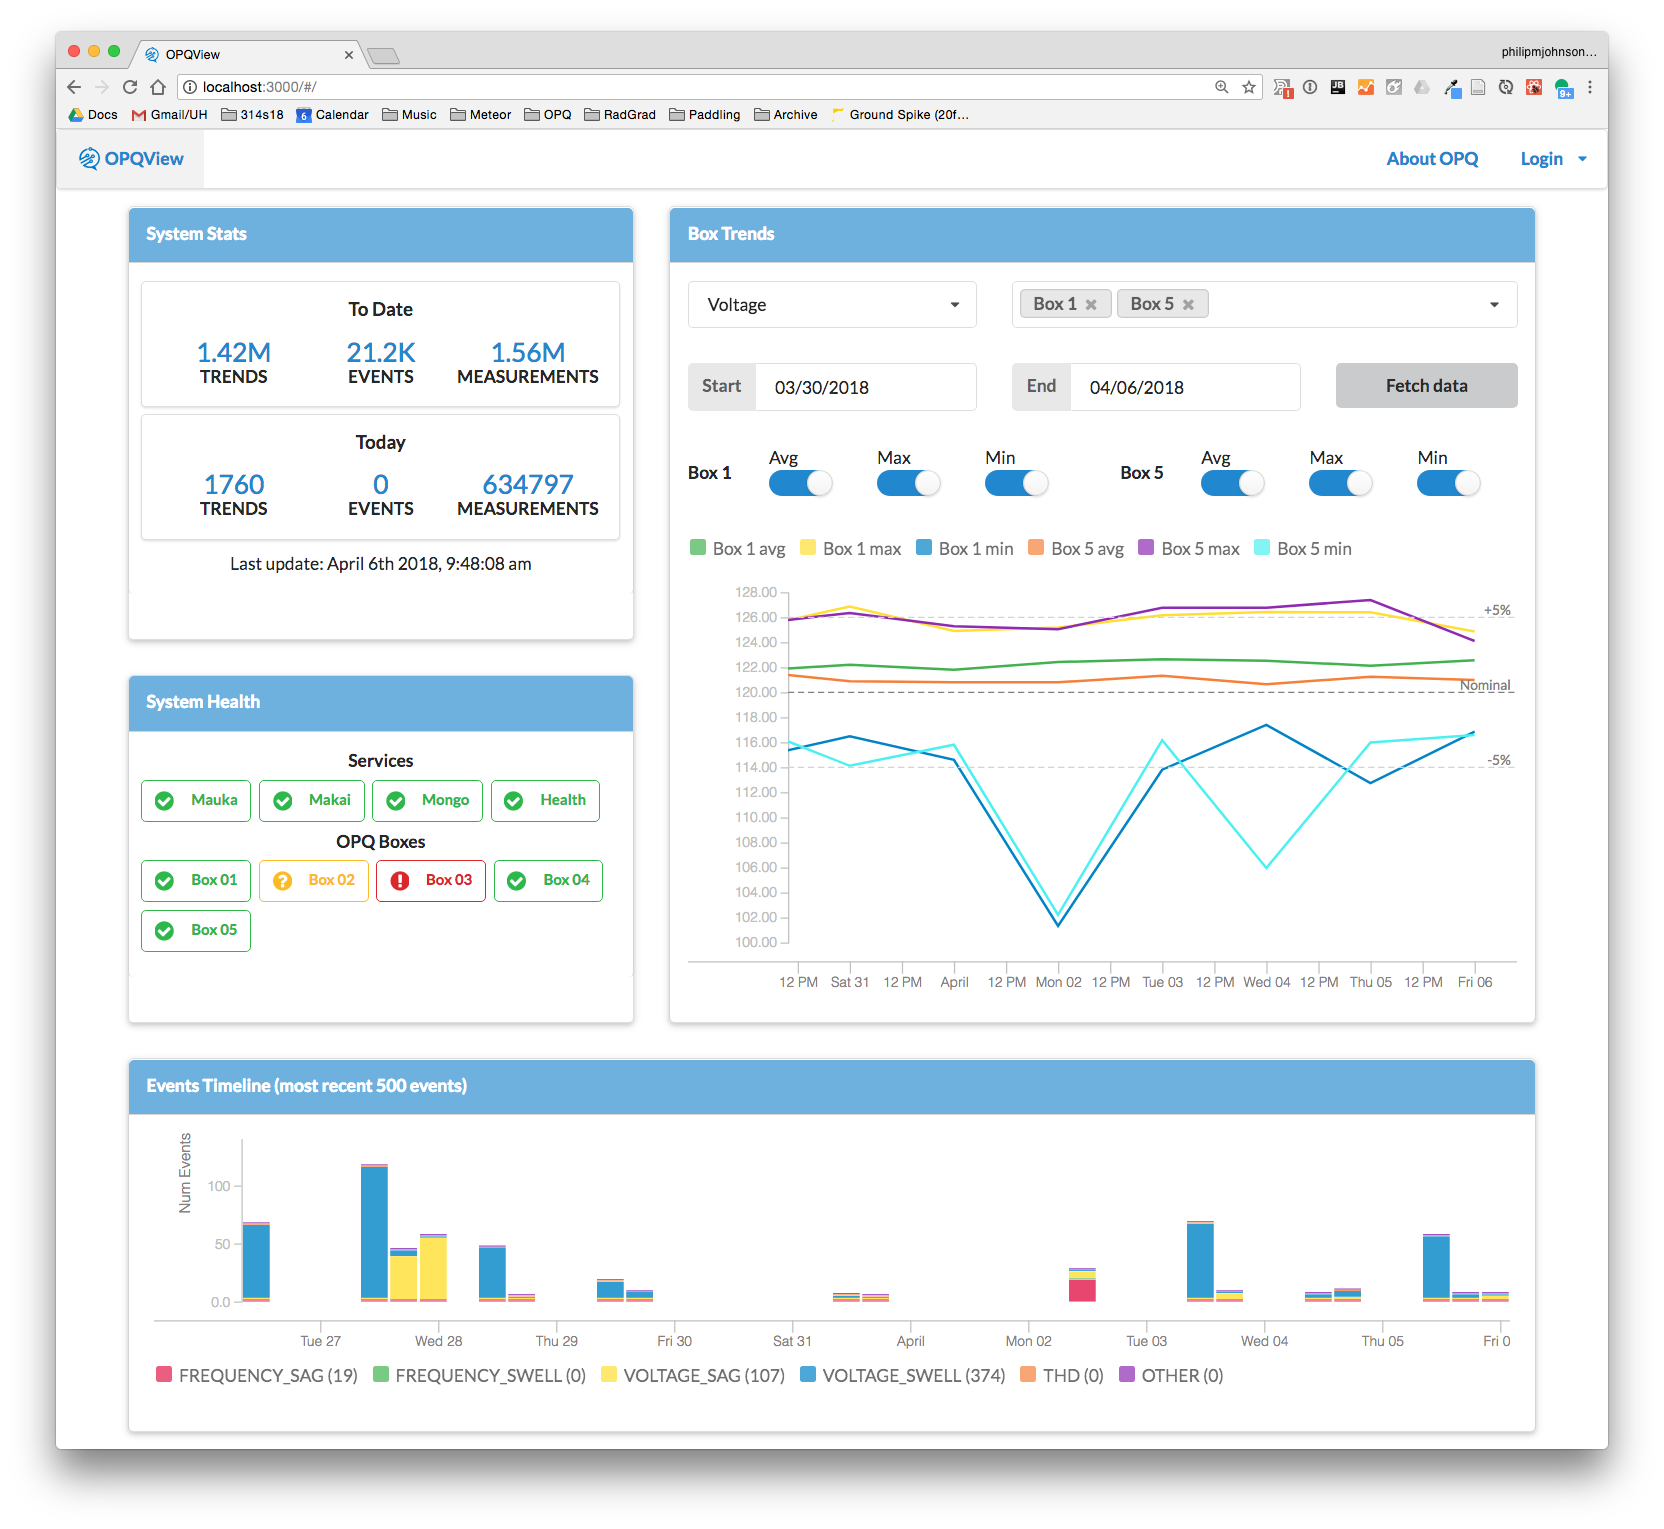
\includegraphics[width=0.6\textwidth]{img/opqview-landing-page.png}
  \end{center}
  \caption{Screenshot of a recent OPQ View build.}
  \label{fig:opq:12}
\end{figure}
